%% ------------------------------------------------------------------------- %%
\chapter{Results and Analysis}
\label{cap:results}

Each dataset pipeline result has all evaluted metrics (AUC, Brier and Logloss), the dataset statistics (described in \ref{dataset-aggregated-statistics}) and the generated hyperparameter space according to Section \ref{sec:hyperparam-space} of Chapter \ref{cap:study-methodology}.

The focus of this Chapter is to give an overview of the main results, how the datasets were clustered, a basic explanation of the statistical theory necessary for the experimental analysis,  some insights about each hyperparameter effect and how sensitive the clustered datasets are to them.


%% ------------------------------------------------------------------------- %%
\section{Single Dataset Experiment}

Each dataset result in the study has the following files:

\begin{enumerate}
    \item \textbf{\code{shape}}: The number of data points $D_i$ and the number of features of both train and test set;
    \item \textbf{\code{analyzer\_info}}: A dictionary with information calculated by the \code{analyzer}. It contains the feature set, what is the target column, an indicator if the dataset contains any categorical variable, and all the categorical features if it has any;
    \item \textbf{\code{openml\_object}}: The original \textit{OpenML} object of the dataset, with its name, description (if it has one), basic attribute information, etc;
    \item \textbf{\code{hp\_tree}}: The generate tree for the dataset, i.e. all nodes of $Hspace_i$;
    \item \textbf{\code{final\_result}}: All the metric results for all combinations of hyperparameters in the hyperparameter tree; Contains the values used for the main analysis.
\end{enumerate}

Each entry of \code{final\_result} contains the evaluators result for both train and test set for all hyperparameters combinations. An example of a single entry in the \code{final\_result} for a specific dataset (\textit{BNG(kr-vs-kp)}, a chess move classification problem) is shown in \ref{lst:krkp-result}.

\begin{lstlisting}[caption={BNG(kr-vs-kp) experiment result for hyperparam combination (0.3, 1700, 10)}, label={lst:krkp-result}]
{'learning_rate': 0.30000000000000004,
'num_estimators': 1700,
'max_depth': 10,
'num_leaves': 1023,
'seed': 42,
'nthread': 32,
'verbose': -1,
'train_result': {'auc_evaluator__target': 0.9963452091395292,
    'logloss_evaluator__target': 0.07025840176806959,
    'brier_score_evaluator__target': 0.020611611004153745},
'test_result': {'auc_evaluator__target': 0.9857593012343584,
    'logloss_evaluator__target': 0.208979460099794,
    'brier_score_evaluator__target': 0.03484311126894392},
}  \end{lstlisting}


Since each dataset has multiple results assigned to it, one can do an \textbf{individual analysis} looking into a single dataset behavior. In this section, a summarized analysis of the \textbf{BNG(kr-vs-kp)} dataset is given as an example. The \textit{BNG(kr-vs-kp)} or "King+Rook versus King+Pawn" is one of the datasets available in the OpenML platform, where the objective is to classify if the white player can win or not (given the board positions determined by the feature values), and it's described in more details in \cite{shapiro1987structured}. The "BNG" means this is an artificially augmented/generated dataset.

\subsection{Individual Hyperparameter Impact}

The first node of the hyperparameter tree only defines single hyperparameters values. By keeping the default LightGBM values for the remaining hyperparameters one can observe the impact of changing a single hyperparameter on each metric of interest. The plot of these values is the classical learning curve used in model tuning to assess hyperparameter effect on model performance. In the Figure \ref{fig:res-ind2} impact of max depth is shown and in \ref{fig:res-ind1} the number of estimators, for the \textit{BNG(kr-vs-kp)} dataset.

\begin{figure}[!h]
    \centering
    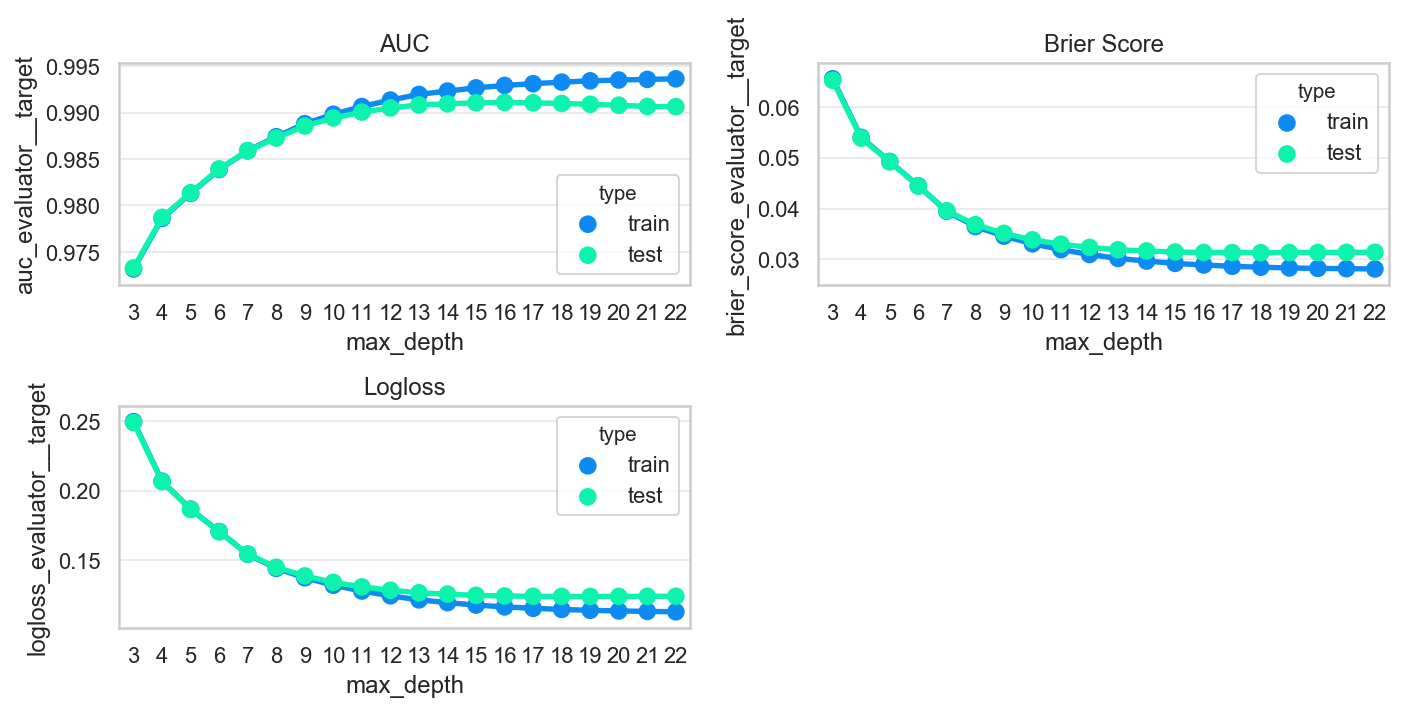
\includegraphics[width=1\textwidth]{res-ind2.png} 
    \caption{Individual impact of \textbf{\code{max\_depth}} on the \textit{BNG(kr-vs-kp)} dataset: one can observe that when $max\_depth > 14$ the model starts to overfit.}
    \label{fig:res-ind2}
\end{figure}

\begin{figure}[!h]
    \centering
    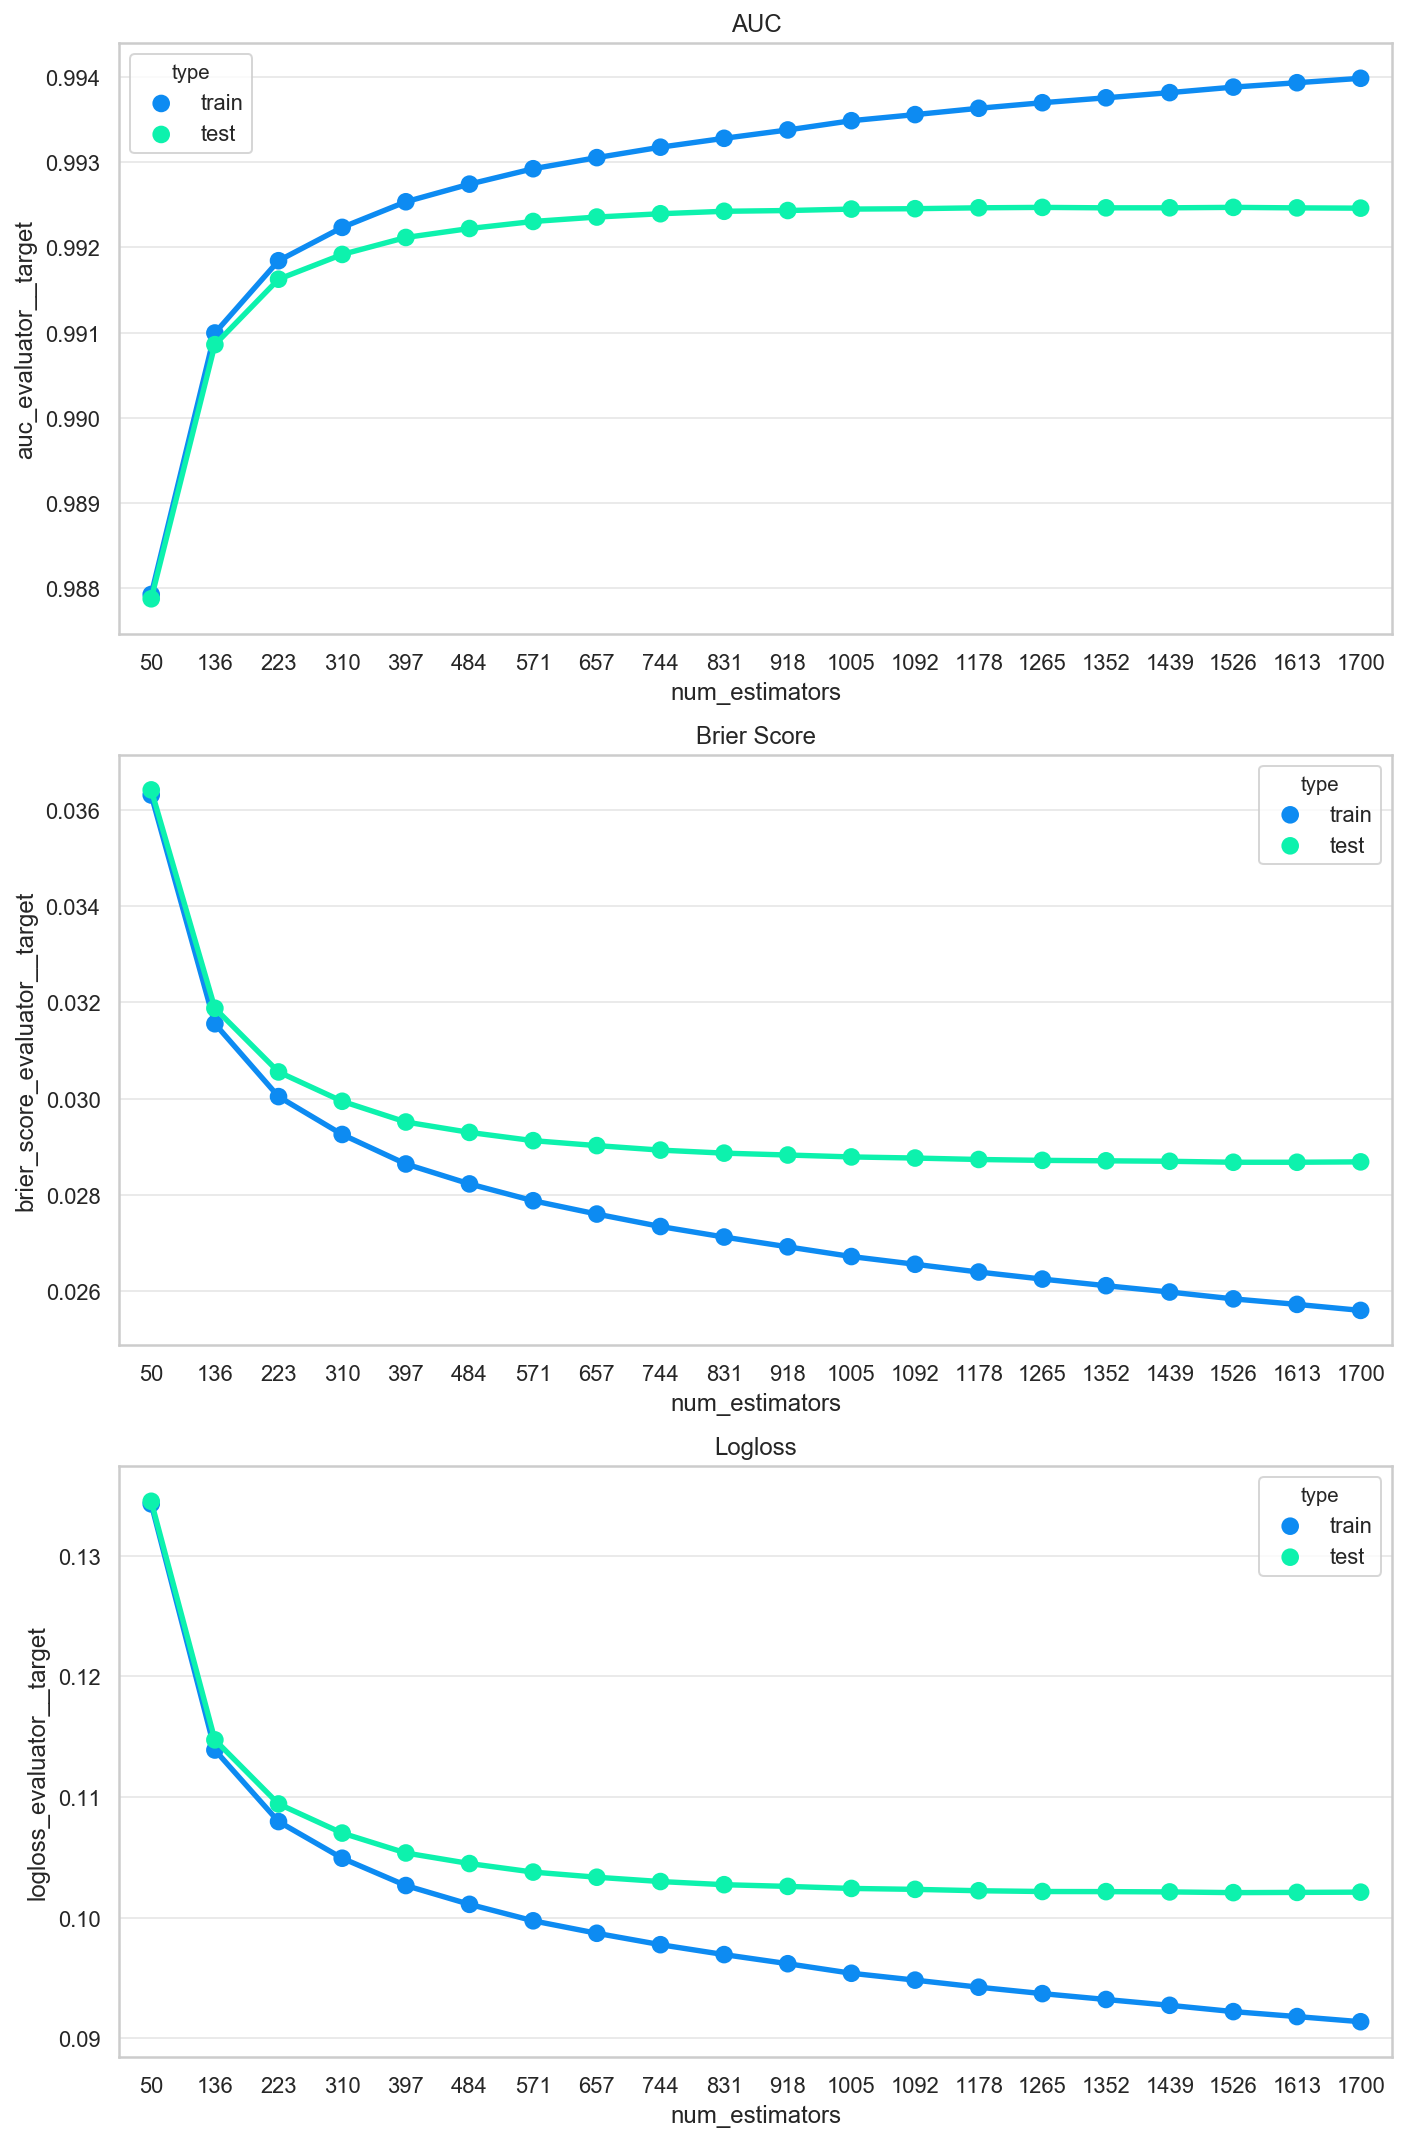
\includegraphics[width=1\textwidth, height=1.2\textwidth]{res-ind1.png} 
    \caption{Individual impact of \textbf{\code{num\_estimators}} on the \textit{BNG(kr-vs-kp)} dataset}
    \label{fig:res-ind1}
\end{figure}

\subsection{Hyperparameter Pairs Impact}

The second node of the hyperparameter tree defines all pairs of possible combinations of hyperparameters. In this study, these combinations are $MD_i \times LR_i$, $MD_i \times NE_i$ and $LR_i \times NE_i$. For example, in Figure \ref{fig:res-mult1} one can see at the same time that a high \textbf{\code{num\_estimators}} combined with lower \textbf{\code{max\_depth}} have higher AUC on the test set (on this specific dataset), but at the same time low \textbf{\code{num\_estimators}} combined with high \textbf{\code{max\_depth}} also achieve high AUC. This is an interesting behavior that repeats in different hyperparameters combinations, and are easily detectable in the final general analysis looking at the treatment effect of each hyperparameter combination.

\begin{figure}[!h]
    \centering
    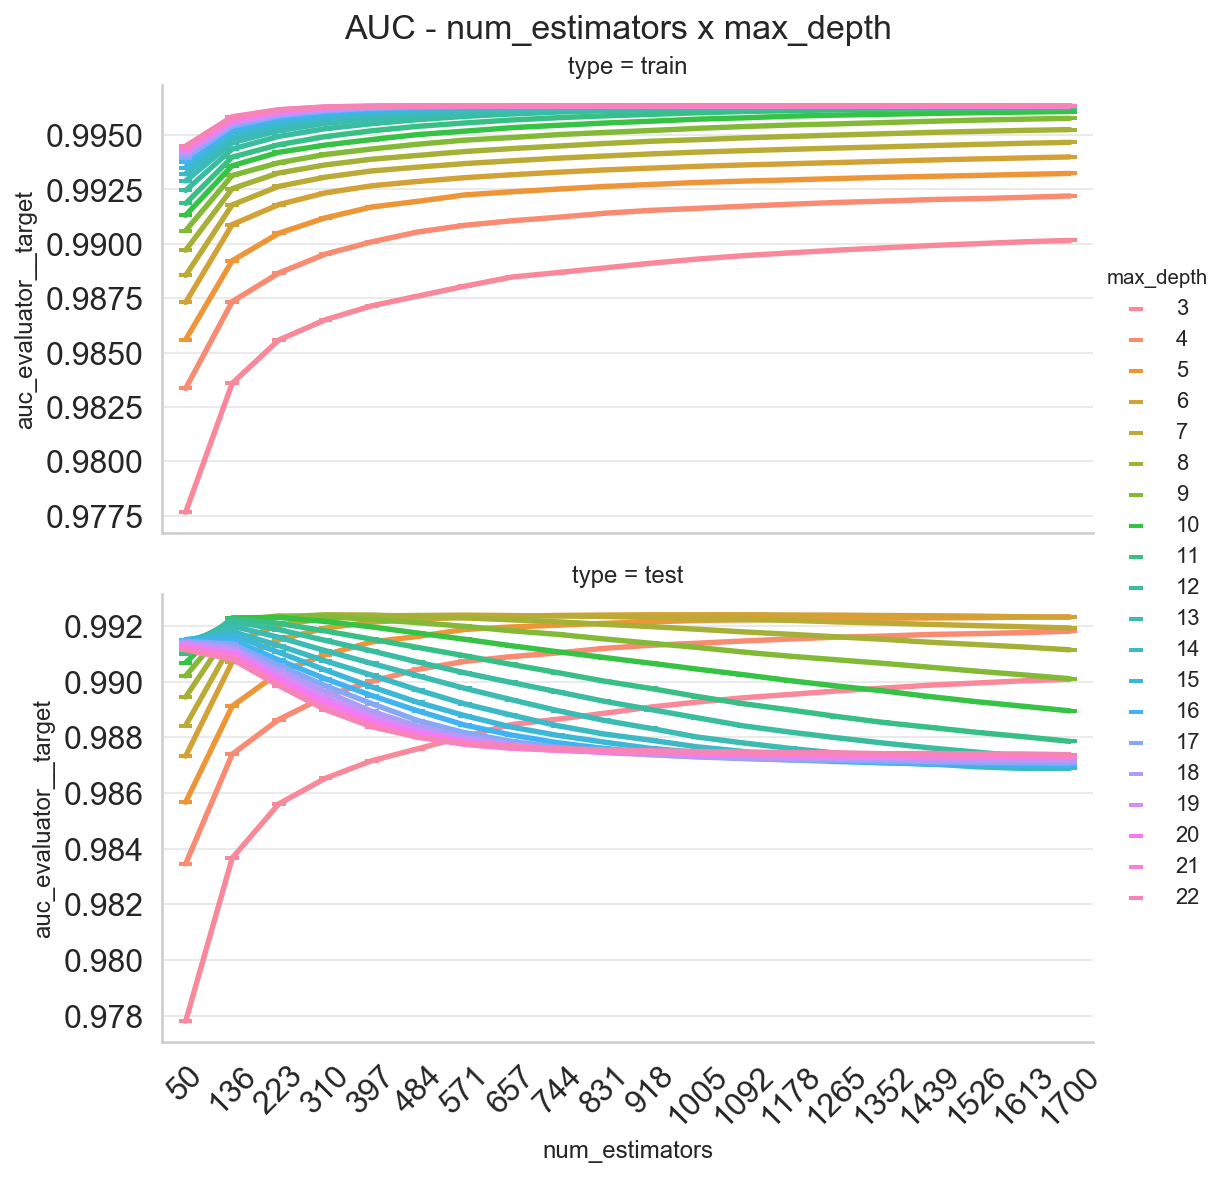
\includegraphics[width=0.8\textwidth]{res-mult1.png} 
    \caption{Pair impact of $MD_i \times NE_i$  on the \textit{BNG(kr-vs-kp)} dataset}
    \label{fig:res-mult1}
\end{figure}

On the other hand, when analyzing \ref{fig:res-mult2} the pair $MD_i \times LR_i$ doesn't show a clear inversion of the hyperparameters impact: one can only conclude that for \textit{BNG(kr-vs-kp)} lower \textbf{\code{max\_depth}} and high \textbf{\code{learning\_rate}} results in higher AUC (keeping the other hyperparameters the same). This is expected since the learning rate doesn't have the same ``overfit relationship'' as maximum depth and number of estimators have (explained in \ref{subsec:max-depth}).

\begin{figure}[!h]
    \centering
    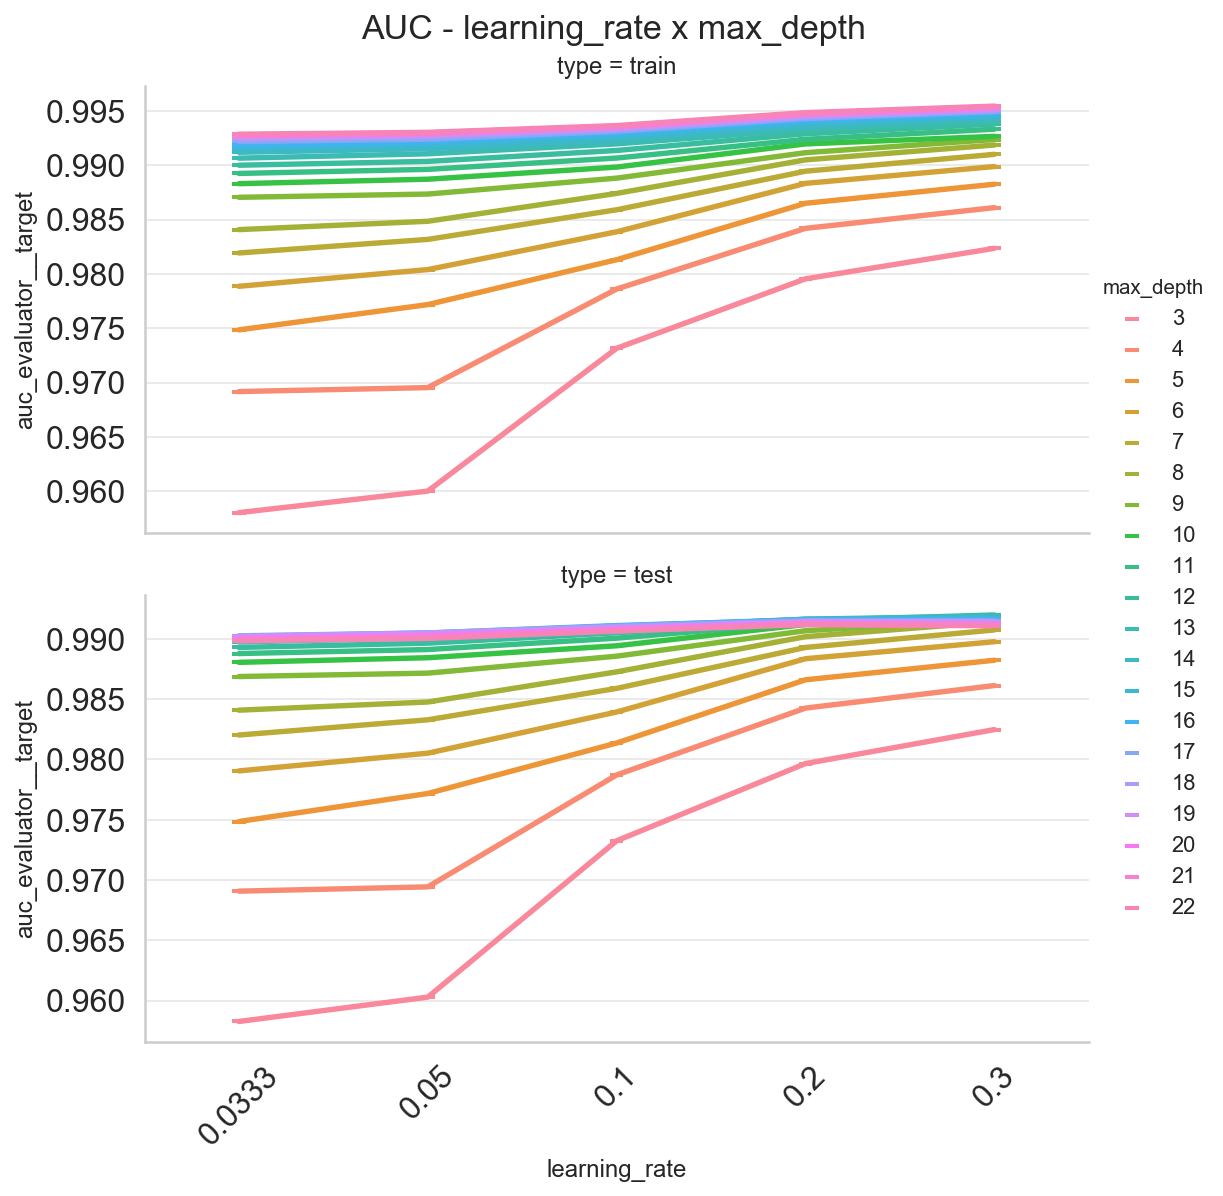
\includegraphics[width=0.8\textwidth]{res-mult2.png}
    \caption{Pair impact of $MD_i \times LR_i$  on the \textit{BNG(kr-vs-kp)} dataset}
    \label{fig:res-mult2}
\end{figure}

\subsection{Hyperparameter Triples Impact}

Finally, each dataset is also run using all possible combinations of the studied hyperparameters, i.e. a classical Grid Search run using \code{num\_estimators}, \code{max\_depth} and \code{learning\_rate}. Results of AUC of the triple impact for  \textit{BNG(kr-vs-kp)} can be seen in Figure \ref{fig:res-all1}.

\begin{figure}[!h]
    \centering
    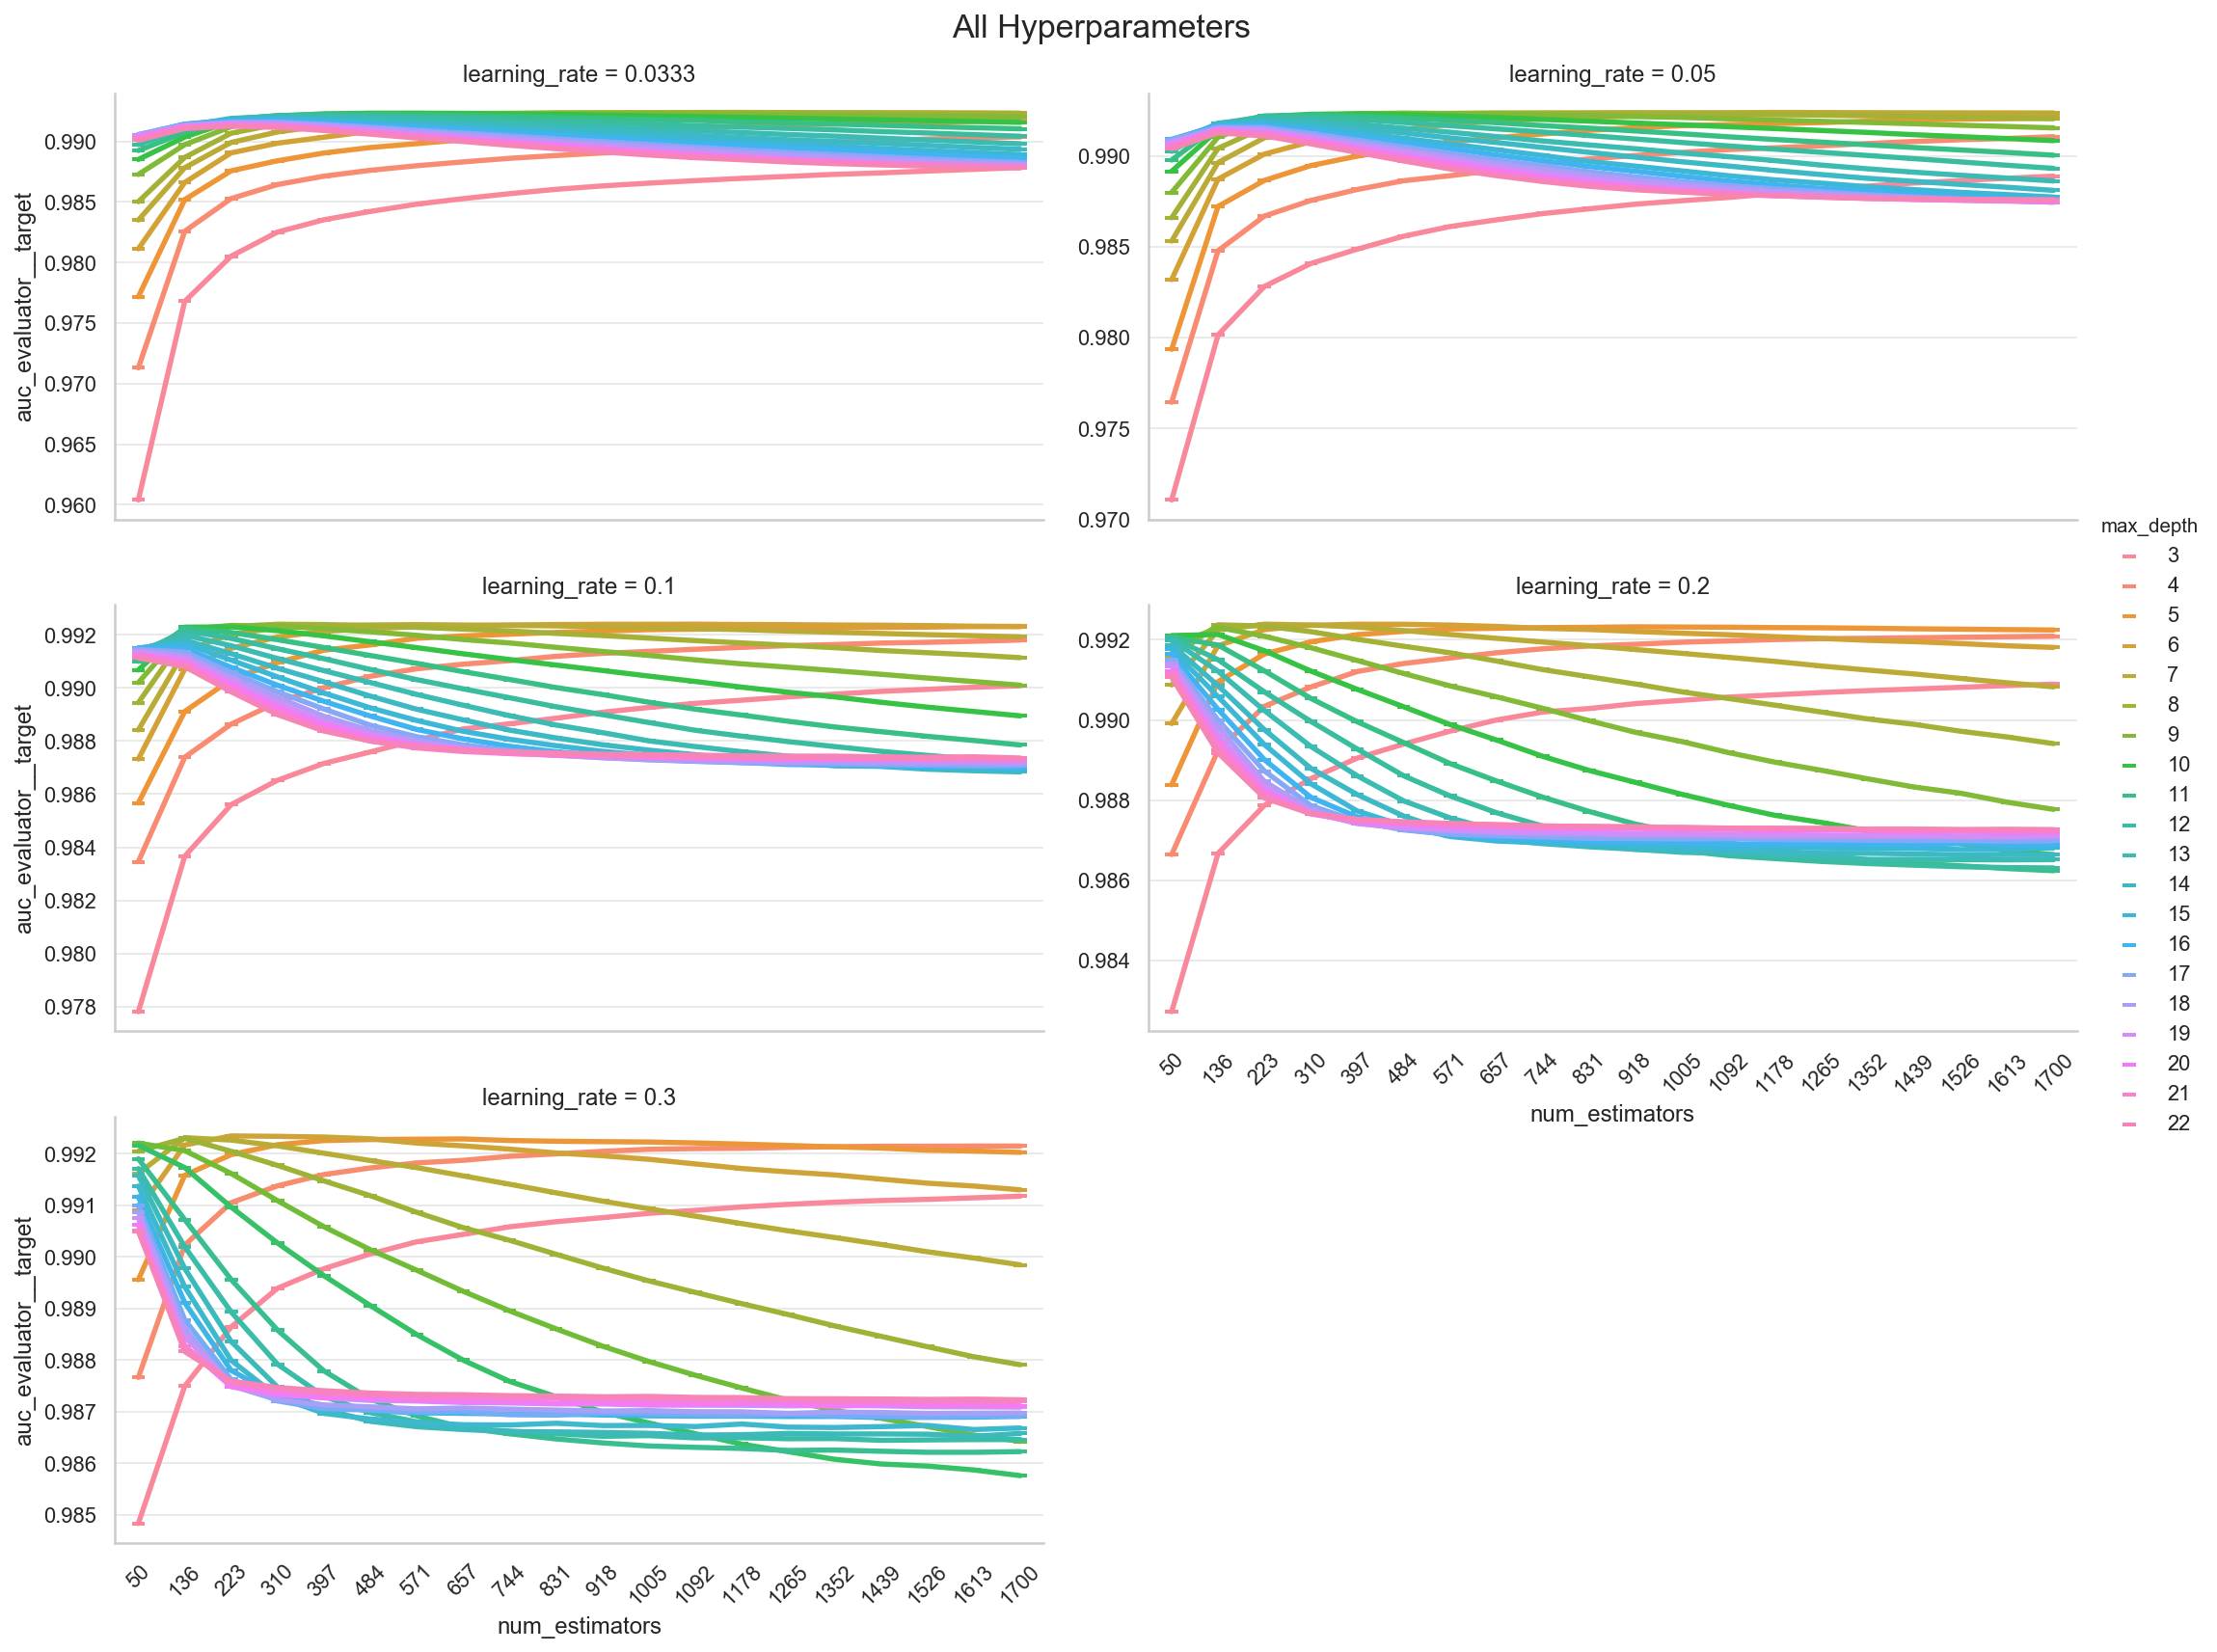
\includegraphics[width=1\textwidth]{res-everything1.png} 
    \caption{Triple impact of hyperparameters on the \textit{BNG(kr-vs-kp)} dataset, showing only \textbf{test} set AUC}
    \label{fig:res-all1}
\end{figure}

One of the inherent difficulties when analyzing these results is due to the high dimensionality of the results: Each experiment has at least the three hyperparameter values, plus three different metrics for each run. In Section \ref{} this problem will be tackled, with an overview of the statistical techniques and analysis performed to compare and obtain insights into the impact on performance metrics.

%% ------------------------------------------------------------------------- %%
\section{Dataset aggregation and clustering}

To tie dataset characteristics to hyperparameters effect in the subsequent analysis, a variety of different measures were calculated in the dataset analysis process, explained in details in Section \ref{dataset-aggregated-statistics} of Chapter \ref{cap:study-methodology}. When analyzing all datasets's features characteristics, useful insights into the data can be found on it. First, a clear conclusion is that proportion of categorical features in the dataset is much higher than  other types (numeric, Boolean or constants), as shown in Figure \ref{fig:dset-pre1}, and that the most common cardinality is two categories for the categorical features\footnote{These categorical features could be encoded as the \textit{Boolean} feature type, or vice-versa. In the study it was decided that Boolean features are columns which had explicitly \textbf{True} and \textbf{False} as values.}, while few features have high cardinality (Figure \ref{fig:dset-pre2}).

\begin{figure}[!h]
    \centering
    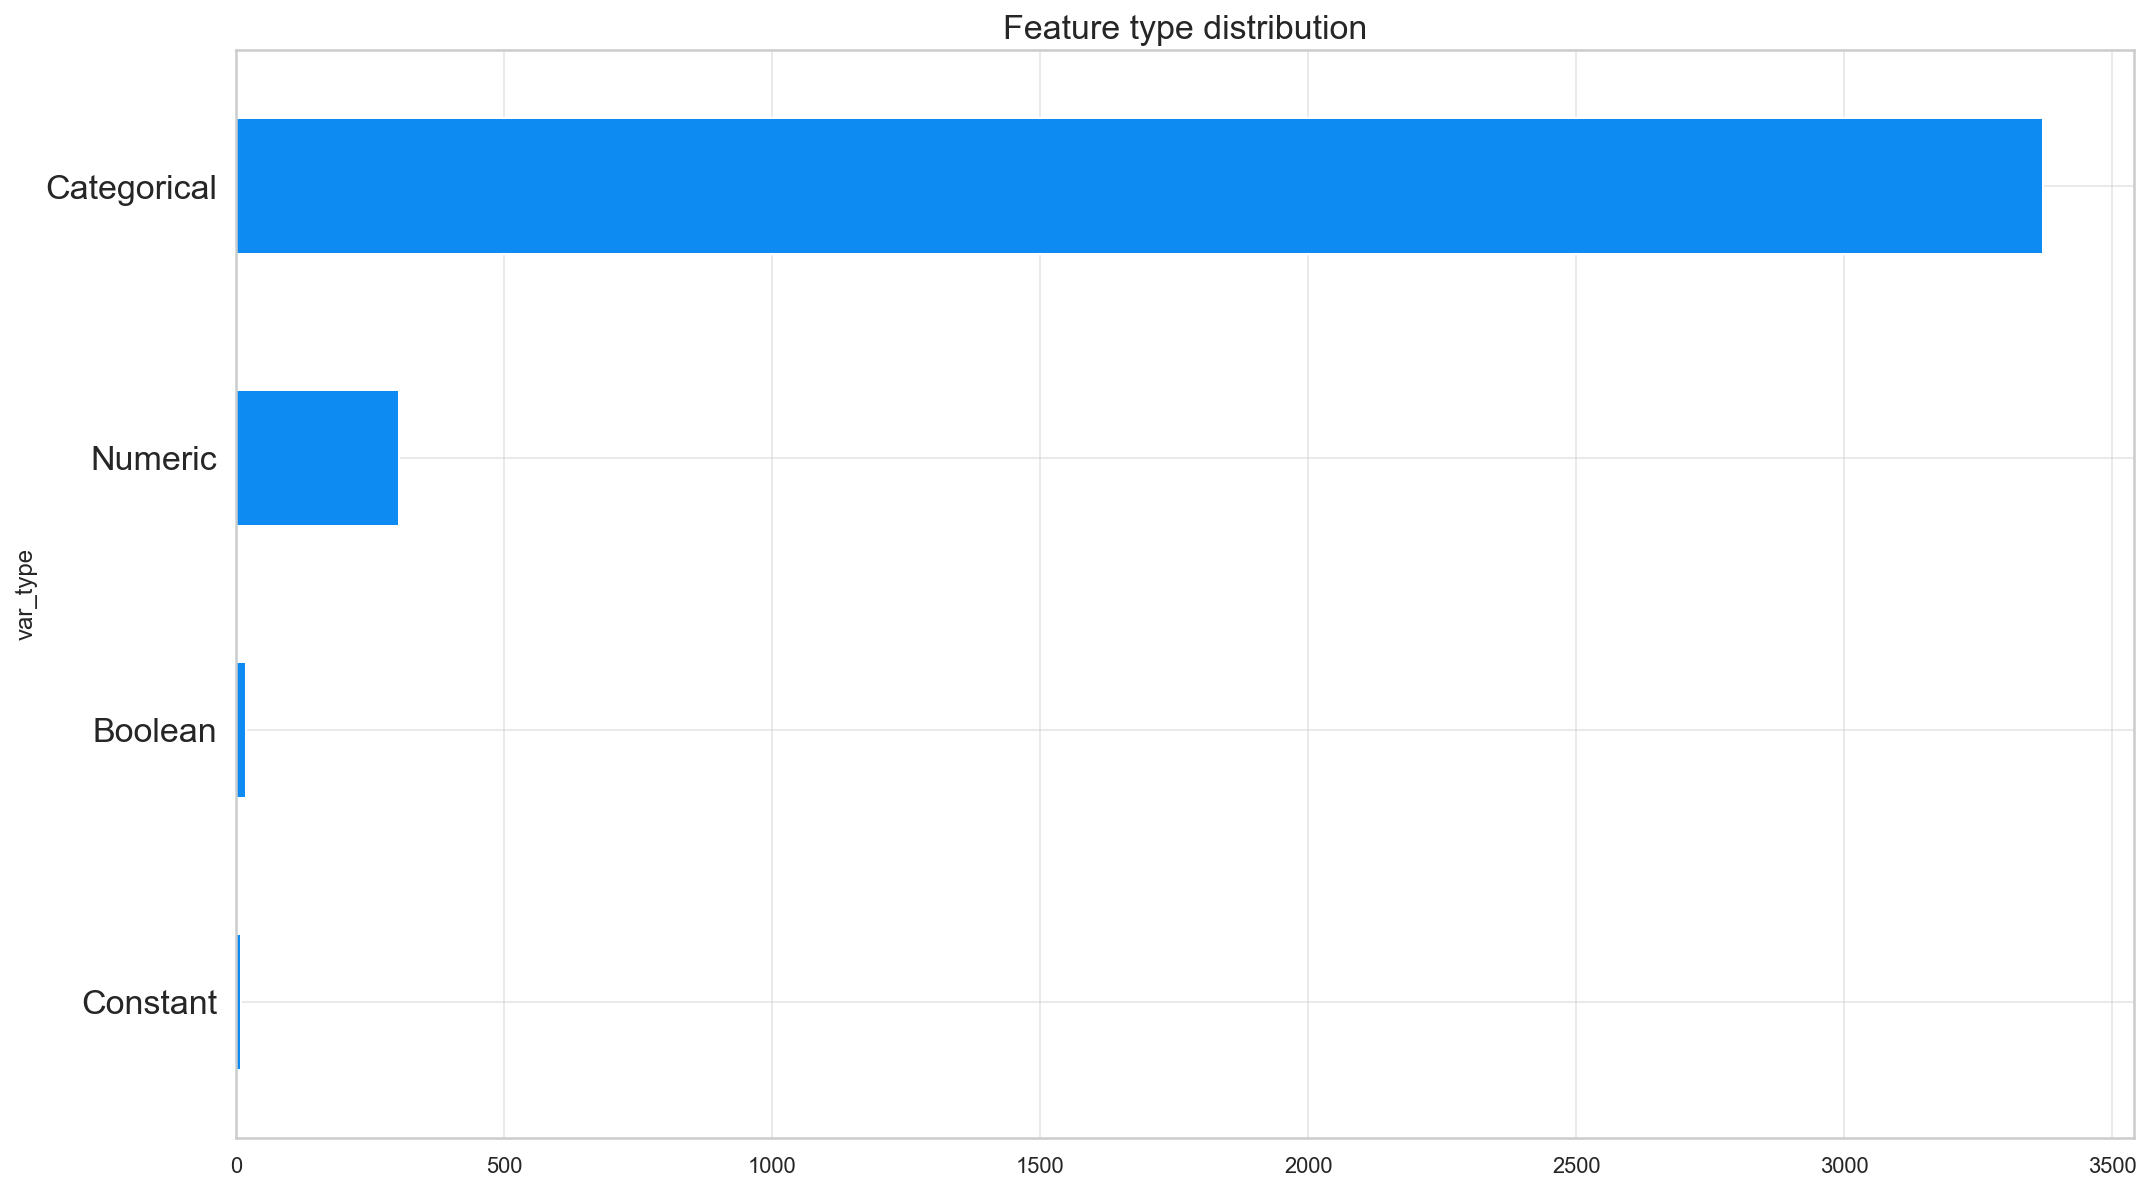
\includegraphics[width=.7\textwidth]{dset-pre1.png} 
    \caption{Feature types of the benchmark datasets}
    \label{fig:dset-pre1}
\end{figure}

\begin{figure}[!h]
    \centering
    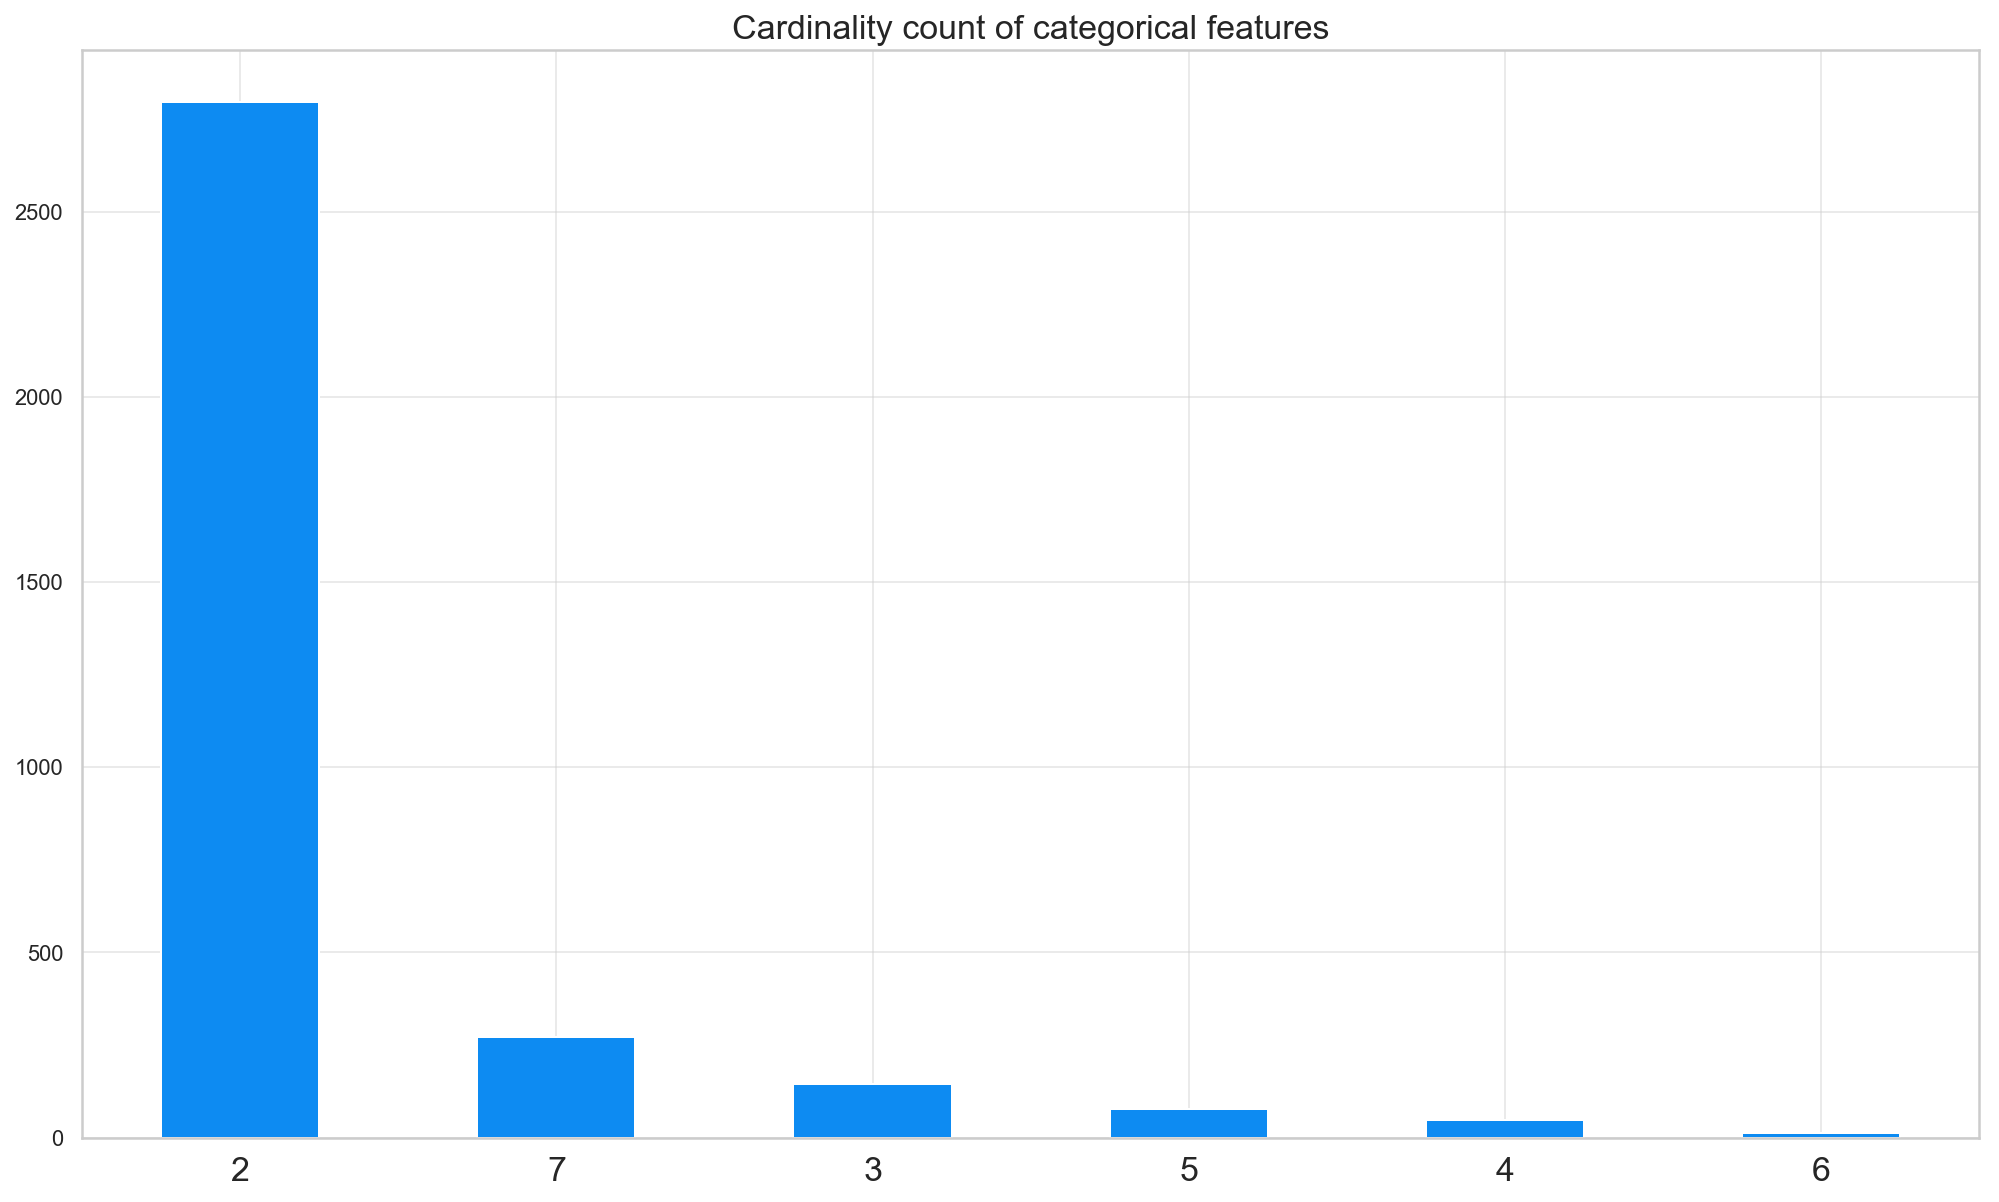
\includegraphics[width=.7\textwidth]{dset-pre2.png} 
    \caption{Cardinality of categorical features of the benchmark datasets}
    \label{fig:dset-pre2}
\end{figure}

With relation to the skewness of the numeric features, most of them have low skewness, with the majority of them having $0$ skewness. This can indicate either that the features themselves do not have innate skewness, or they've been processed different techniques to normalize and remove skewness, like a logarithmic transformation, cubic root transformation, etc. The distribution can be seen in Figure \ref{fig:dset-pre3}.

\begin{figure}[!h]
    \centering
    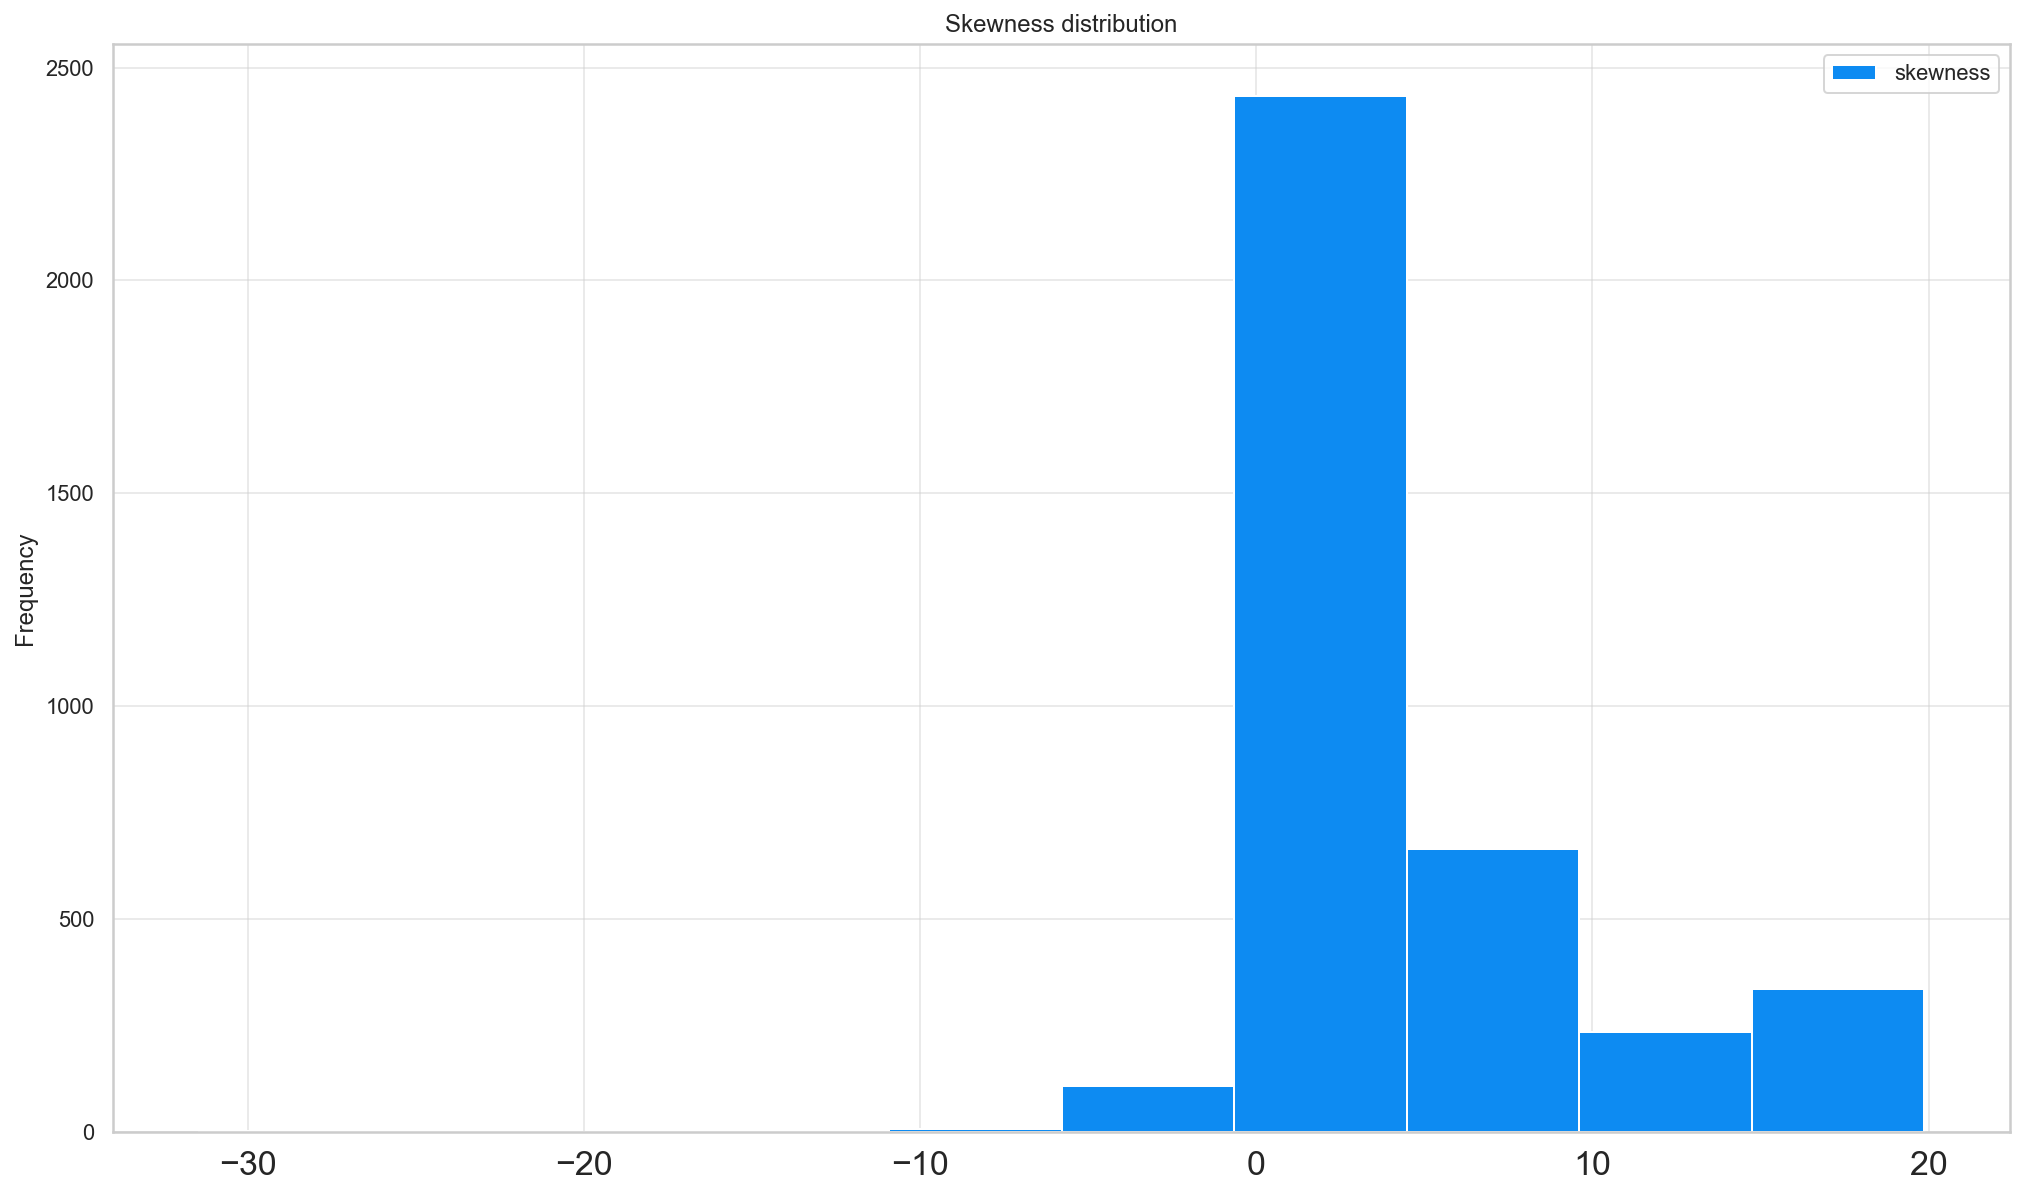
\includegraphics[width=.7\textwidth]{dset-pre3.png}
    \caption{Skewness distribution of the numeric features in the dataset}
    \label{fig:dset-pre3}
\end{figure}

\subsection{Aggregation}

Since the granularity of the statistics are feature-wise, all datasets were subjected to an aggregation process which combines the feature-wise statistics into \textit{dataset aggregated characteristics}. The objective of this aggregation is to represent each dataset considered in the study into a point in a high dimensional space, which gives power to perform a multitude of transformations and comparisons, and in the case of this study, a clustering by the similarity of the datasets according to these aggregated values. For each dataset, the following aggregations are made:

\begin{itemize}
    \item \textbf{\code{num\_rows}}: Number of rows in the dataset, i.e. the number of instances of $D_i$;
    \item \textbf{\code{num\_features}}: Number of features in the dataset;
    \item \textbf{\code{mean\_skewness}}: $0$ if there's no numeric features in the dataset, otherwise the mean of the skewness of the numeric features;
    \item \textbf{\code{mean\_variance}}: The mean of the \textit{variance} of categorical features, where the variance concept is the one described at Section \ref{dataset-aggregated-statistics};
    \item \textbf{\code{num\_categorical}}: How many categorical features the dataset has;
    \item \textbf{\code{sum\_cardinality\_over\_categorical}}: Let $K$ be the set of categorical features of the dataset, and $Cardinality_K$ the sum of the cardinality of all $k\in K$. Then, this aggregation is defined as $\frac{Cardinality_K}{|K| + 1}$, which is simply the "\textit{mean}" of cardinality in the dataset. The $+1$ is to avoid error with datasets which do not have categorical features;
    \item \textbf{\code{categorical\_ratio}}: Proportion of categorical features in the dataset;
    \item \textbf{\code{numeric\_ratio}}: Proportion of numeric features;
    \item \textbf{\code{boolean\_ratio}}: Proportion of Boolean features;
    \item \textbf{\code{constant\_ratio}}: Proportion of constant features.
\end{itemize}


After this transformation each dataset $D_i$ is now represented by a $\mathcal{P}_i \in \mathbb{R}^{10}$ where each component of the multidimensional point represents one of the aggregated characteristics calculated above. To visualize these multidimensional points, a t-SNE projection (dimensionality reduction technique, more details in \cite{maaten2008visualizing}) on two dimensions is shown in Figure \ref{fig:tsne-1}.

\begin{figure}[!h]
    \centering
    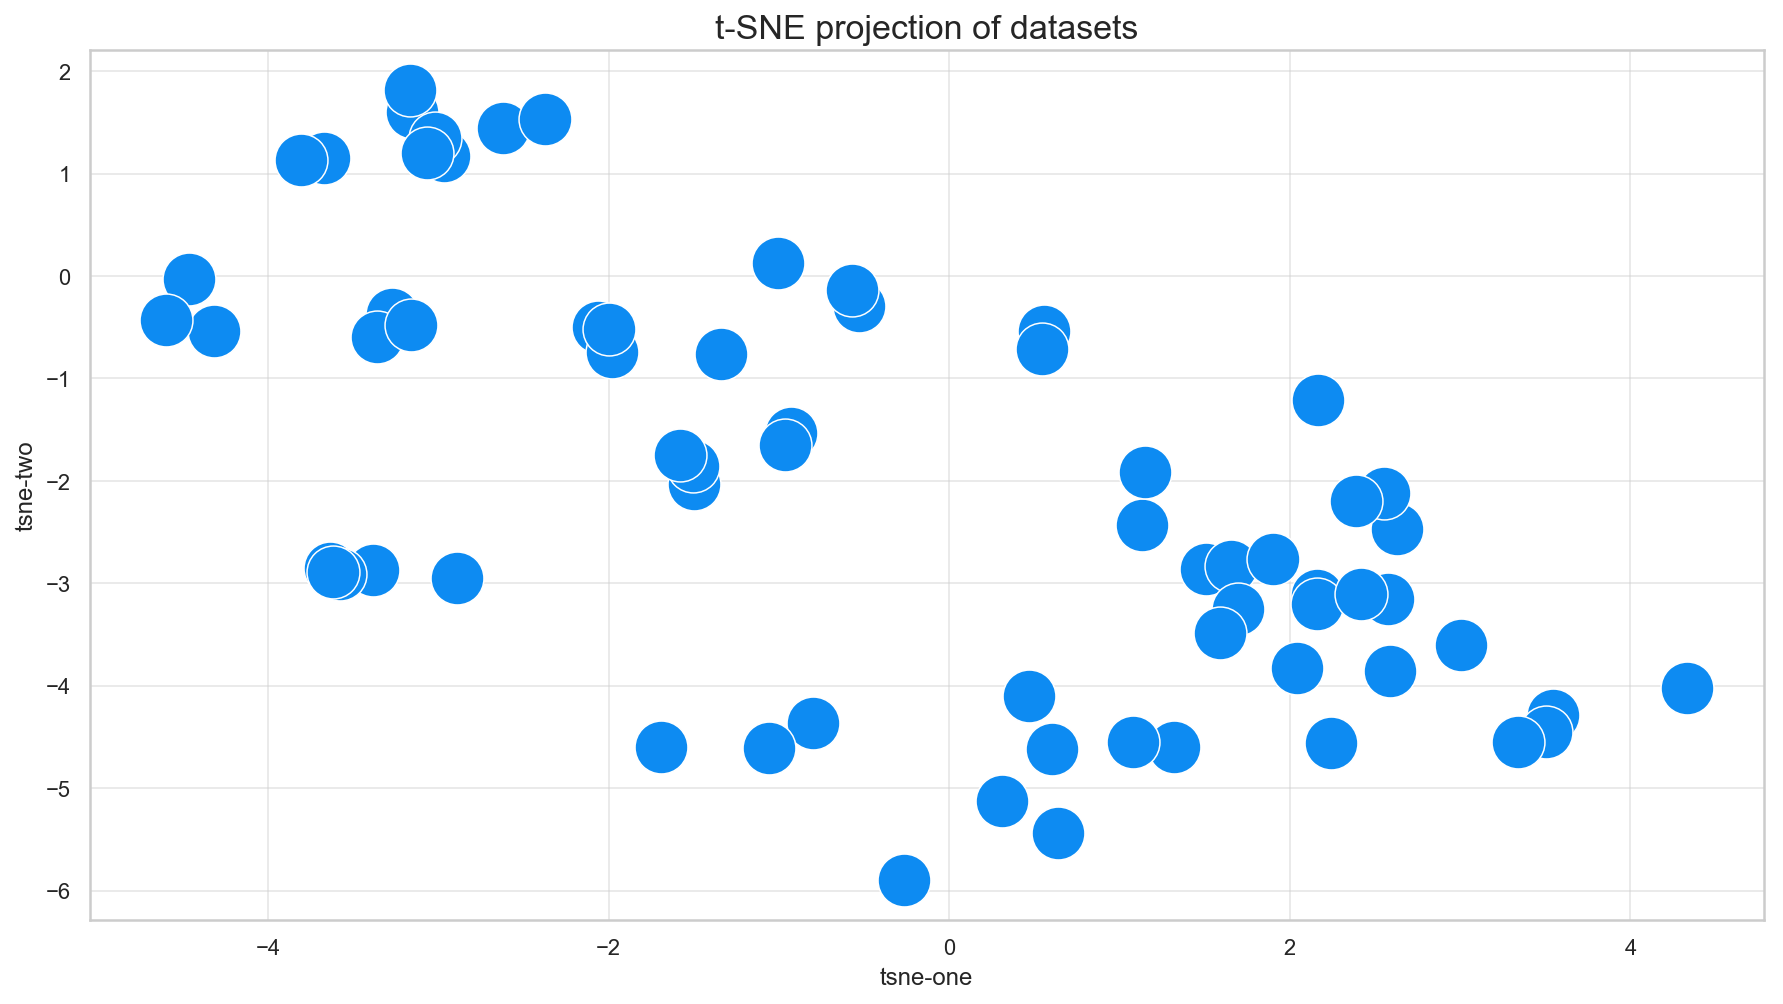
\includegraphics[width=1\textwidth]{tsne1.png}
    \caption{t-SNE projection of all $\mathcal{P}_i$}
    \label{fig:tsne-1}
\end{figure}

The aggregated characteristics were designed in a way to encompass both the proportion of feature types in the dataset and the absolute size of the dataset. The \code{*ratio} aggregations are done to compare multiple datasets regardless on the absolute numeric value of features it has, but on the ratio of the feature types. On the other hand, the absolute features like \code{num\_rows} captures the absolute size of the data. For example, a simple analysis using \code{num\_rows}, \code{num\_features} and \code{categorical\_ratio} could yield interesting insights and a way to bundle similar datasets together based on the proportion of categorical features, controlling for both the number of data points and the number of features. 

Finally, there's also explicit emphasis on characteristics regarding numeric and categorical features, which are of interest in this study (more information about the premisses about it on Section \ref{dataset-aggregated-statistics} of Chapter \ref{cap:study-methodology}). The mean of skewness aggregation can be used to control (in the experimental design sense) for datasets with similar distribution of skewed or not numerical features, while the mean of variance, the number of categorical features and the "\textit{mean}" of cardinality describes important information regarding the categorical aspect of the dataset.  

\subsection{Clustering Strategy}

To analyze all experiments based on similar dataset characteristics, the decided approach was to perform a simple clustering technique, instead of manually selecting which datasets are similar by looking at the aggregated characteristics by hand. Using the aggregated characteristics explained on the last section, a clustering approach on the points $\mathcal{P}_i$ generates clusters based on those characteristics.

\begin{figure}[!h]
    \centering
    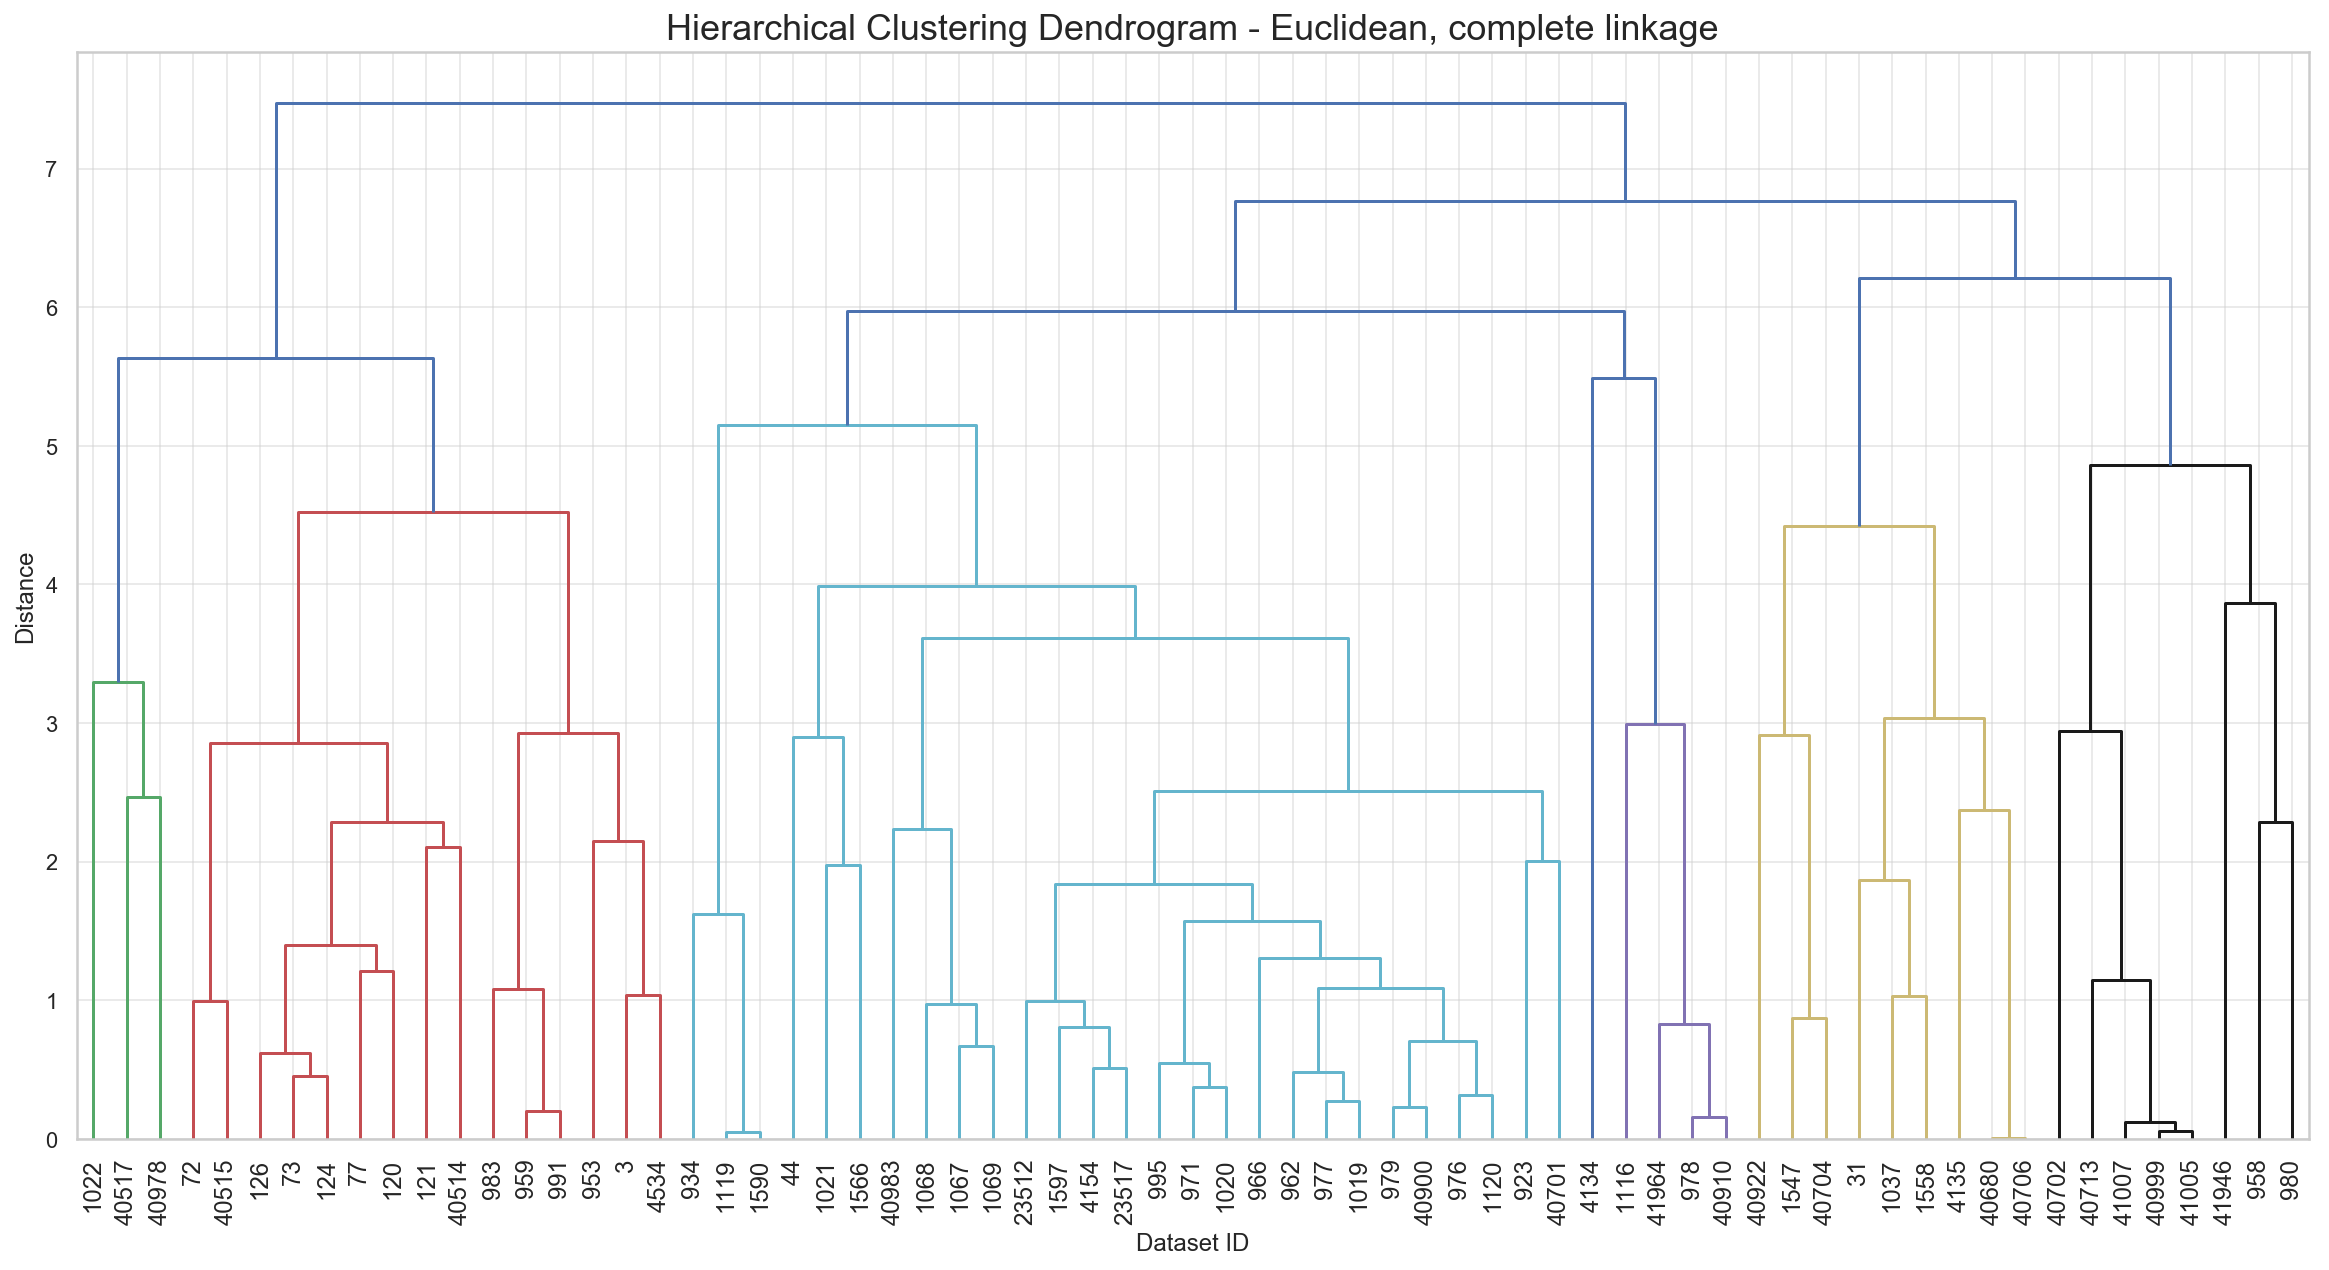
\includegraphics[width=1\textwidth]{dendrogram.png}
    \caption{Dendrogram of the old clustering method}
    \label{fig:dendrogram}
\end{figure}

After some initial experimentation, the chosen clustering approach was to use the well known K-means algorithm, with $k=6$ clusters. K-means is a very simple algorithm which reduces the data to \textit{centroids}, and resulted in reasonable clusters for this study. The other tested technique was to use agglomerative hierarchical clustering, and choose the number of clusters by analyzing the resulting dendrogram (the dendrogram for the hierarchical clustering is shown in Figure \ref{fig:dendrogram}). However, this technique generated an uneven number of datasets in each cluster, more than K-means, so the K-means was chosen. It's important to note that the algorithms and the number of clusters chosen here can highly impact the subsequent analysis of the experiment results. The objective is not to create a generic analysis that could work with any possible dataset, but to actually measure the impact of hyperparameters into specific clusters which follow a similar distribution of the aggregated characteristics.

After the K-means procedure, the assigned clusters can be seen in the t-SNE projection in Figure \ref{fig:tsne-2}, where each color represents a different cluster. Even though the number of $\mathcal{P}_i$ in each cluster isn't uniform, the clustering assignment is more intuitive, albeit in reduced dimensionality. As an observation note, the two t-SNE projections (Figure \ref{fig:tsne-1} and  \ref{fig:tsne-2}) are different because the embeddings in low dimension change when new data is introduced. In this case, the centroids were also added to the dataset before using t-SNE.

\begin{figure}[!h]
    \centering
    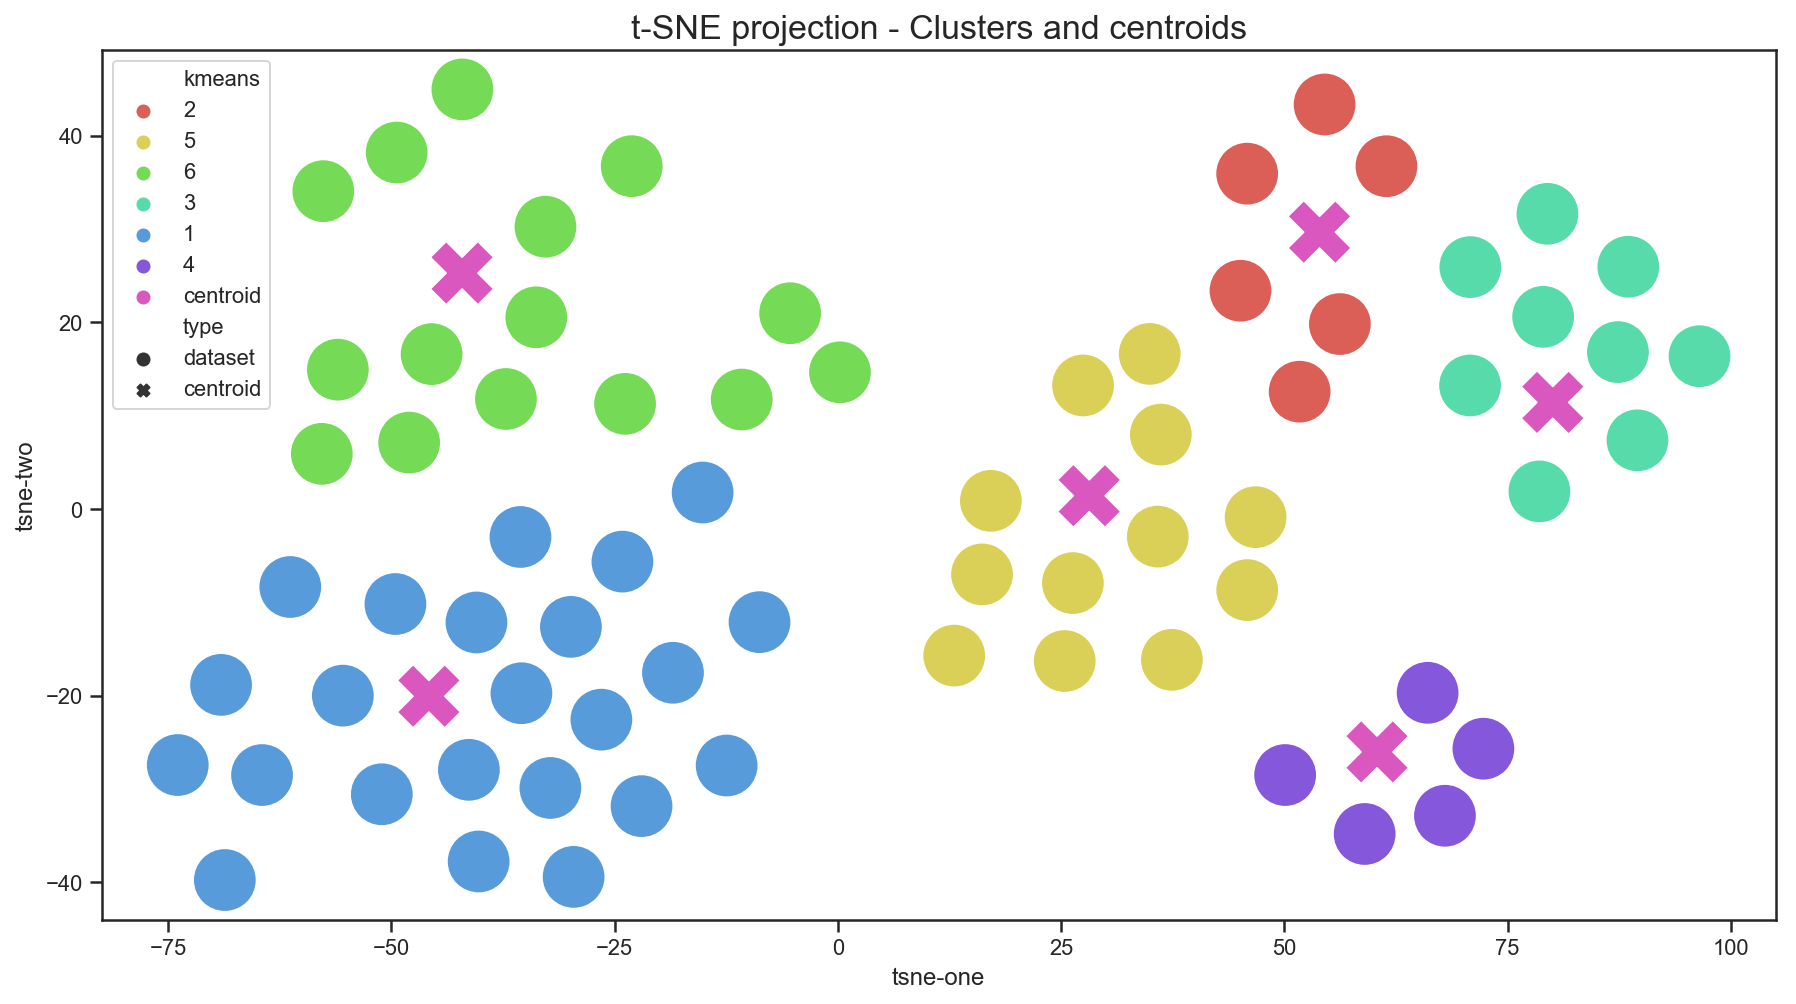
\includegraphics[width=1\textwidth]{tsne2.png}
    \caption{t-SNE projection with the assigned clusters and the centroids}
    \label{fig:tsne-2}
\end{figure}

To understand better the behavior and semantic of each dataset of clusters, manual analysis of the datasets in each one was performed. As an example, the datasets names of Cluster 2 and 3 are in Table \ref{table:1}. From a superficial analysis on the content of each dataset, one can see that most of the datasets in Cluster 2 have a high number of categorical features, while datasets in Cluster 3 are all synthetically augmented, i.e. Bayesian Network Generated (\textit{BNG}) and have a very high number of rows.

\begin{table}[h!]
    \centering
    \begin{tabular}{||c c||} 
     \hline
     Cluster 2 & Cluster 3 \\ [0.5ex] 
     \hline\hline
     \textit{kr-vs-kp} & \textit{BNG(kr-vs-kp)} \\
     \textit{splice} & \textit{BNG(labor,nominal,1000000)} \\
     \textit{mfeat-pixel} & \textit{BNG(breast-cancer,nominal,1000000)} \\
     \textit{PhishingWebsites} & \textit{BNG(mushroom)} \\
     \textit{20\_newsgroups.drift} & \textit{BNG(colic.ORIG,nominal,1000000)} \\
     \textit{Internet-Advertisements} & \textit{BNG(credit-a,nominal,1000000)} \\
     & \textit{BNG(credit-g,nominal,1000000)} \\
     & \textit{BNG(credit-g)} \\[1ex] 
     \hline
    \end{tabular}
    \caption{Datasets from Cluster 2 and Cluster 3}
    \label{table:1}
\end{table}

Using ridgeline plots is another way to understand the meaning of each cluster. By calculating the distribution of the aggregated characteristics over each cluster and plotting them in the same scale against each other, it's possible to evaluate if the clustering makes sense. In total there are $10$ ridgeline plots, one for each aggregated characteristic. Here two of them are shown: In Figure \ref{fig:joyplot-1} and Figure \ref{fig:joyplot-2} the ridgeline plots for \code{categorical\_ratio} and \code{mean\_skewness} can be seen. It's easy to see that Cluster 2 datasets have a very high categorical ratio with very little variance, i.e. almost all of the datasets in this cluster contains a high proportion of categorical features. Clusters 1 and 6 have the lowest proportion of categorical features amongst all Clusters. Another conclusion is that Cluster 6 contains more skewed features, as its distribution is skewed towards high \code{mean\_skewness} values.

All the remaining ridgeline plots are available on the appendix \ref{}.

\begin{figure}[!h]
    \centering
    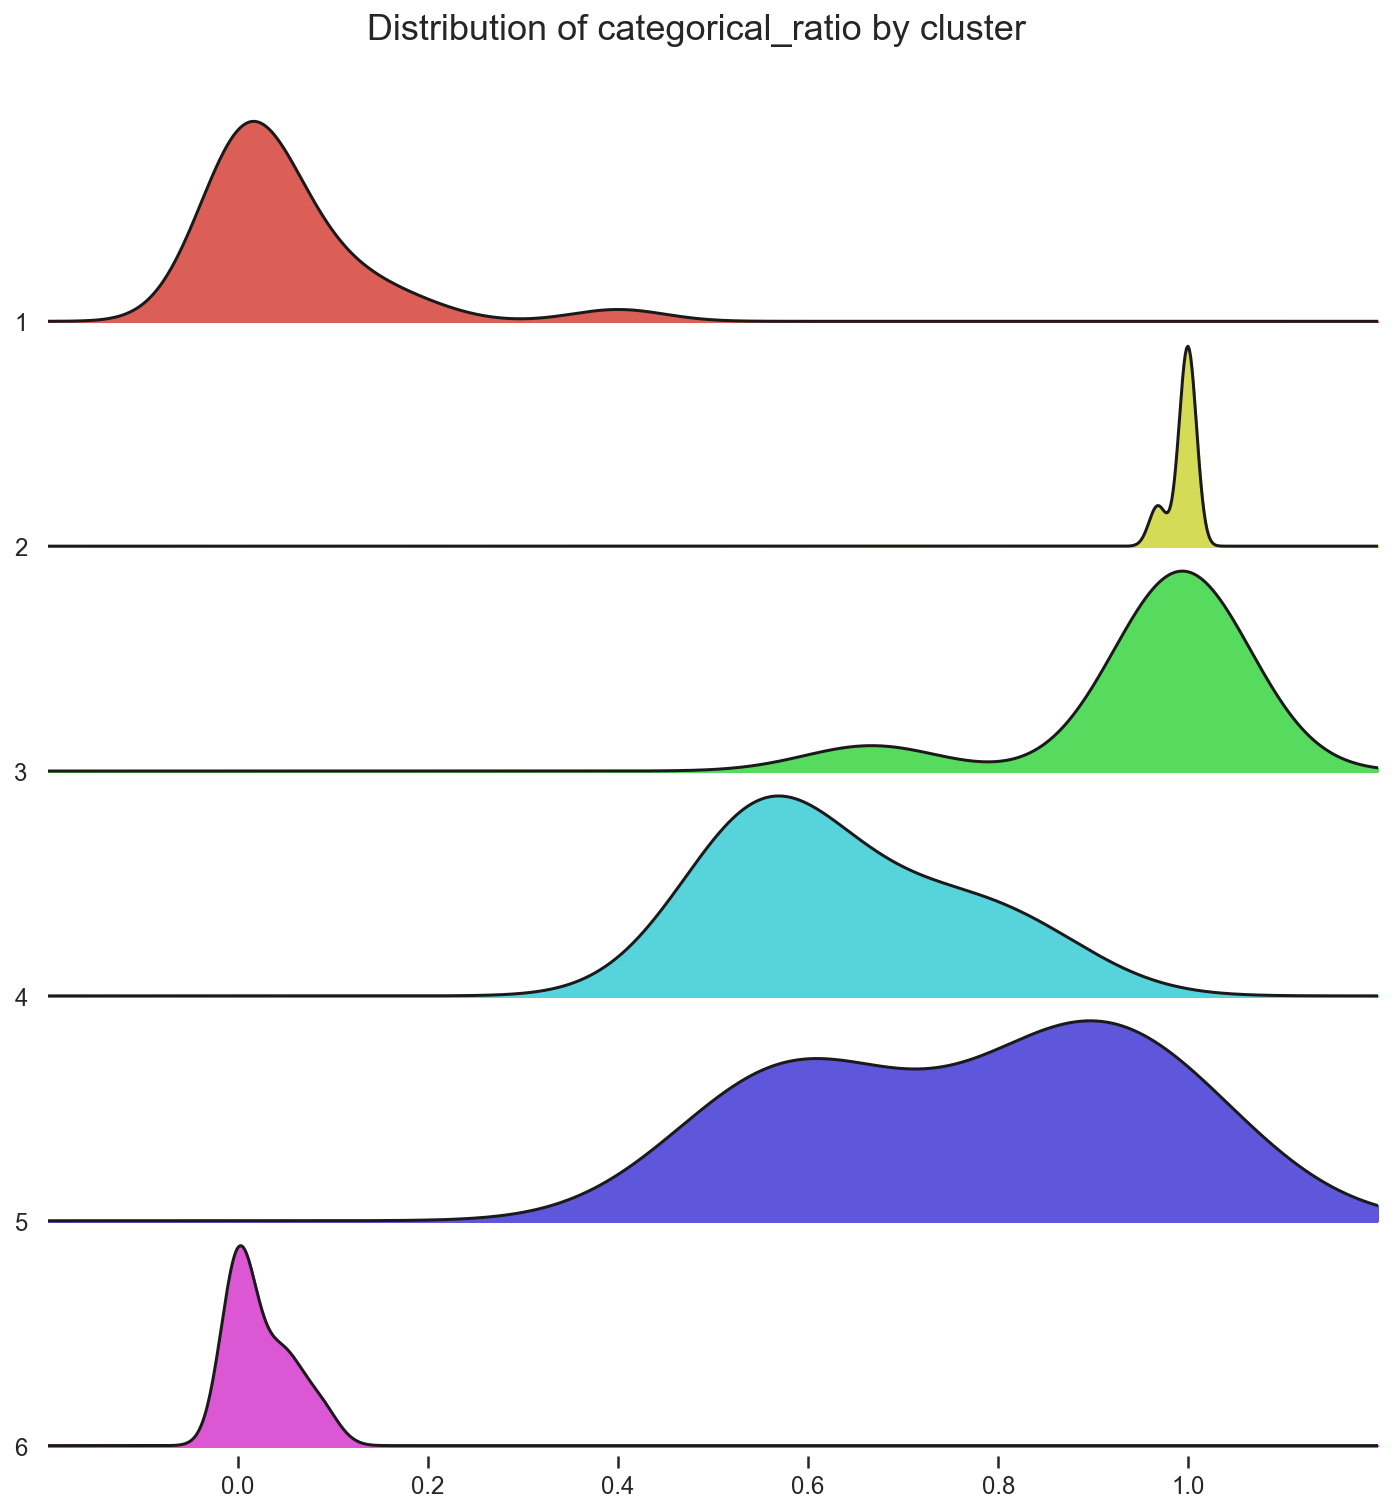
\includegraphics[width=.7\textwidth, height=.7\textwidth]{joyplot1.png}
    \caption{Ridgeline plot of \code{categorical\_ratio}. Clusters are represented by different colors}
    \label{fig:joyplot-1}
\end{figure}

\begin{figure}[!h]
    \centering
    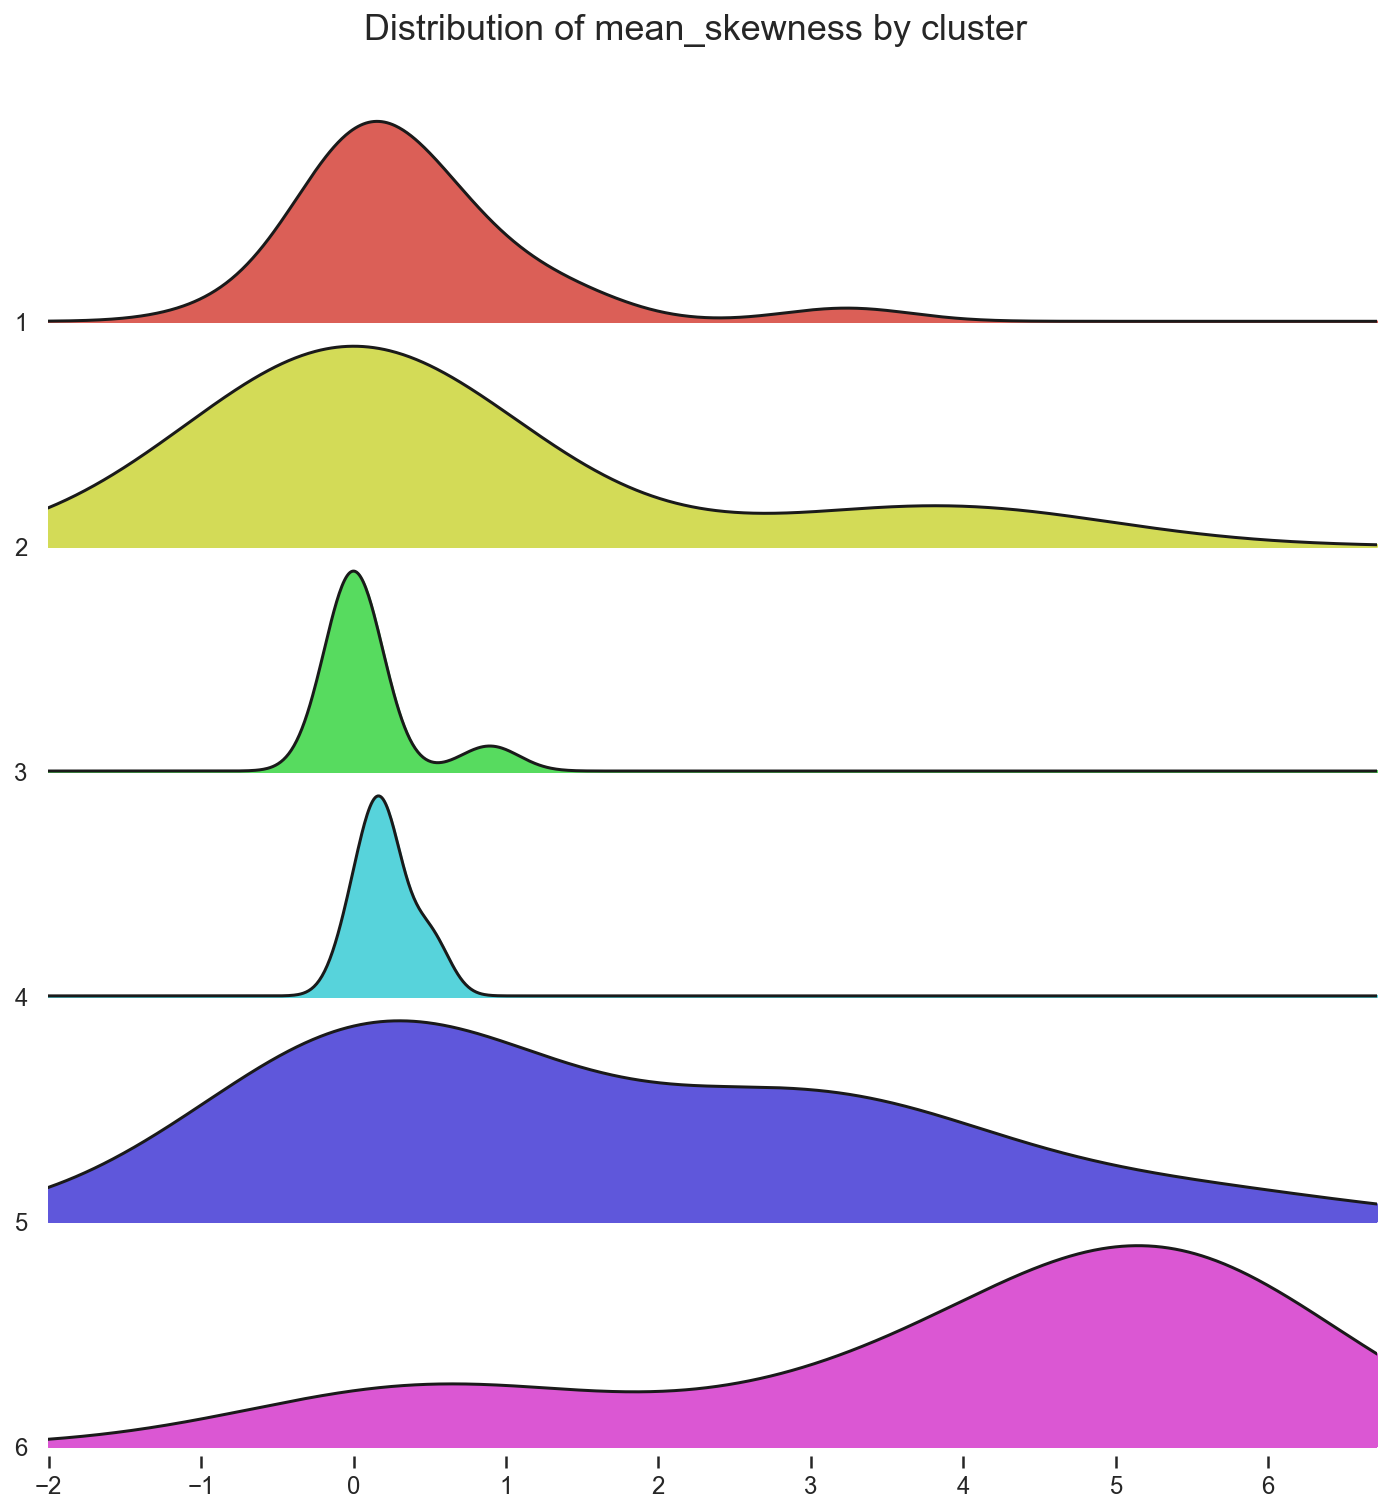
\includegraphics[width=.7\textwidth, height=.7\textwidth]{joyplot2.png}
    \caption{Ridgeline plot of \code{mean\_skewness}. Clusters are represented by different colors}
    \label{fig:joyplot-2}
\end{figure}


%% ------------------------------------------------------------------------- %%
\section{Experiment analysis}

The experimental analysis is performed on each cluster, therefore a common metric must be used when comparing multiple dataset's results. In fact, one of the objectives is to analyze the impact of changing selected hyperparameters on the specified performance metrics of classification tasks. For this part of the analysis, instead of looking directly into the performance metrics of AUC, Logloss and Brier Score, a \textit{delta} from the baseline metric $\delta$ is defined.

\subsection{\texorpdfstring{$\delta_{metric}$}{delta} definition}

The reason to not directly use the performance metrics when comparing different models under the same hyperparameters changes is that the objective of the study doesn't takes into account the actual performance of a given dataset, but actually how much each hyperparameter affects the performance metrics (for better or worse). For example, it doesn't matter in this case if dataset $A$ has a higher AUC than dataset $B$ under a new hyperparameter value $h$, but actually if the increase or decrease in performance of both datasets $A$ and $B$ are significant for hyperparameter value $h$. 

Another problem that can be avoided by the following definition of a $\delta_{metric}$ is the fact that it captures relative changes, instead of the absolute value of the metric; e.g. a dataset with almost constant $0.9$ AUC value will have a $\delta_{AUC}$ equal to $0$ most of the time, and will be treated as equal as a dataset with constant low AUC (e.g. $0.55$): the actual absolute value of the AUC doesn't matter.

LightGBM has a default set of values for its hyperparameters and the ones analyzed in this study  are defined below. As an observation, the correct default value for \code{max\_depth} is $-1$ because it's unlimited on LightGBM, as mentioned in Section \ref{gbm-hyperparams}; However, because the \code{num\_leaves} default is 31 and this approximately results in a balanced tree with depth 5.

\begin{itemize}
    \item LR = \{0.1\}
    \item NE = \{100\}
    \item MD = \{5\}
\end{itemize}

The baseline metrics are defined, for each dataset $D_i$, as the performance metrics (\textit{AUC, Logloss} and \textit{Brier Score}, more details in Section \ref{classification-metrics}) obtained on the test set using the LightGBM model trained with the parameters as close as possible to the default hyperparameter values above. The $\delta_{metric}$ is then just the difference between a given new metric and the baseline metric. It's interpretation depends on the performance metric being analyzed: in the case of AUC, a positive $\delta_{AUC}$ means a higher AUC than baseline (a better result), a negative one means a lower AUC than baseline (worse result), and $0$ an equal performance in terms of AUC. For both the Brier Score and Logloss the interpretation is the opposite, as in these metrics the lower the better.

\begin{figure}[!h]
    \centering
    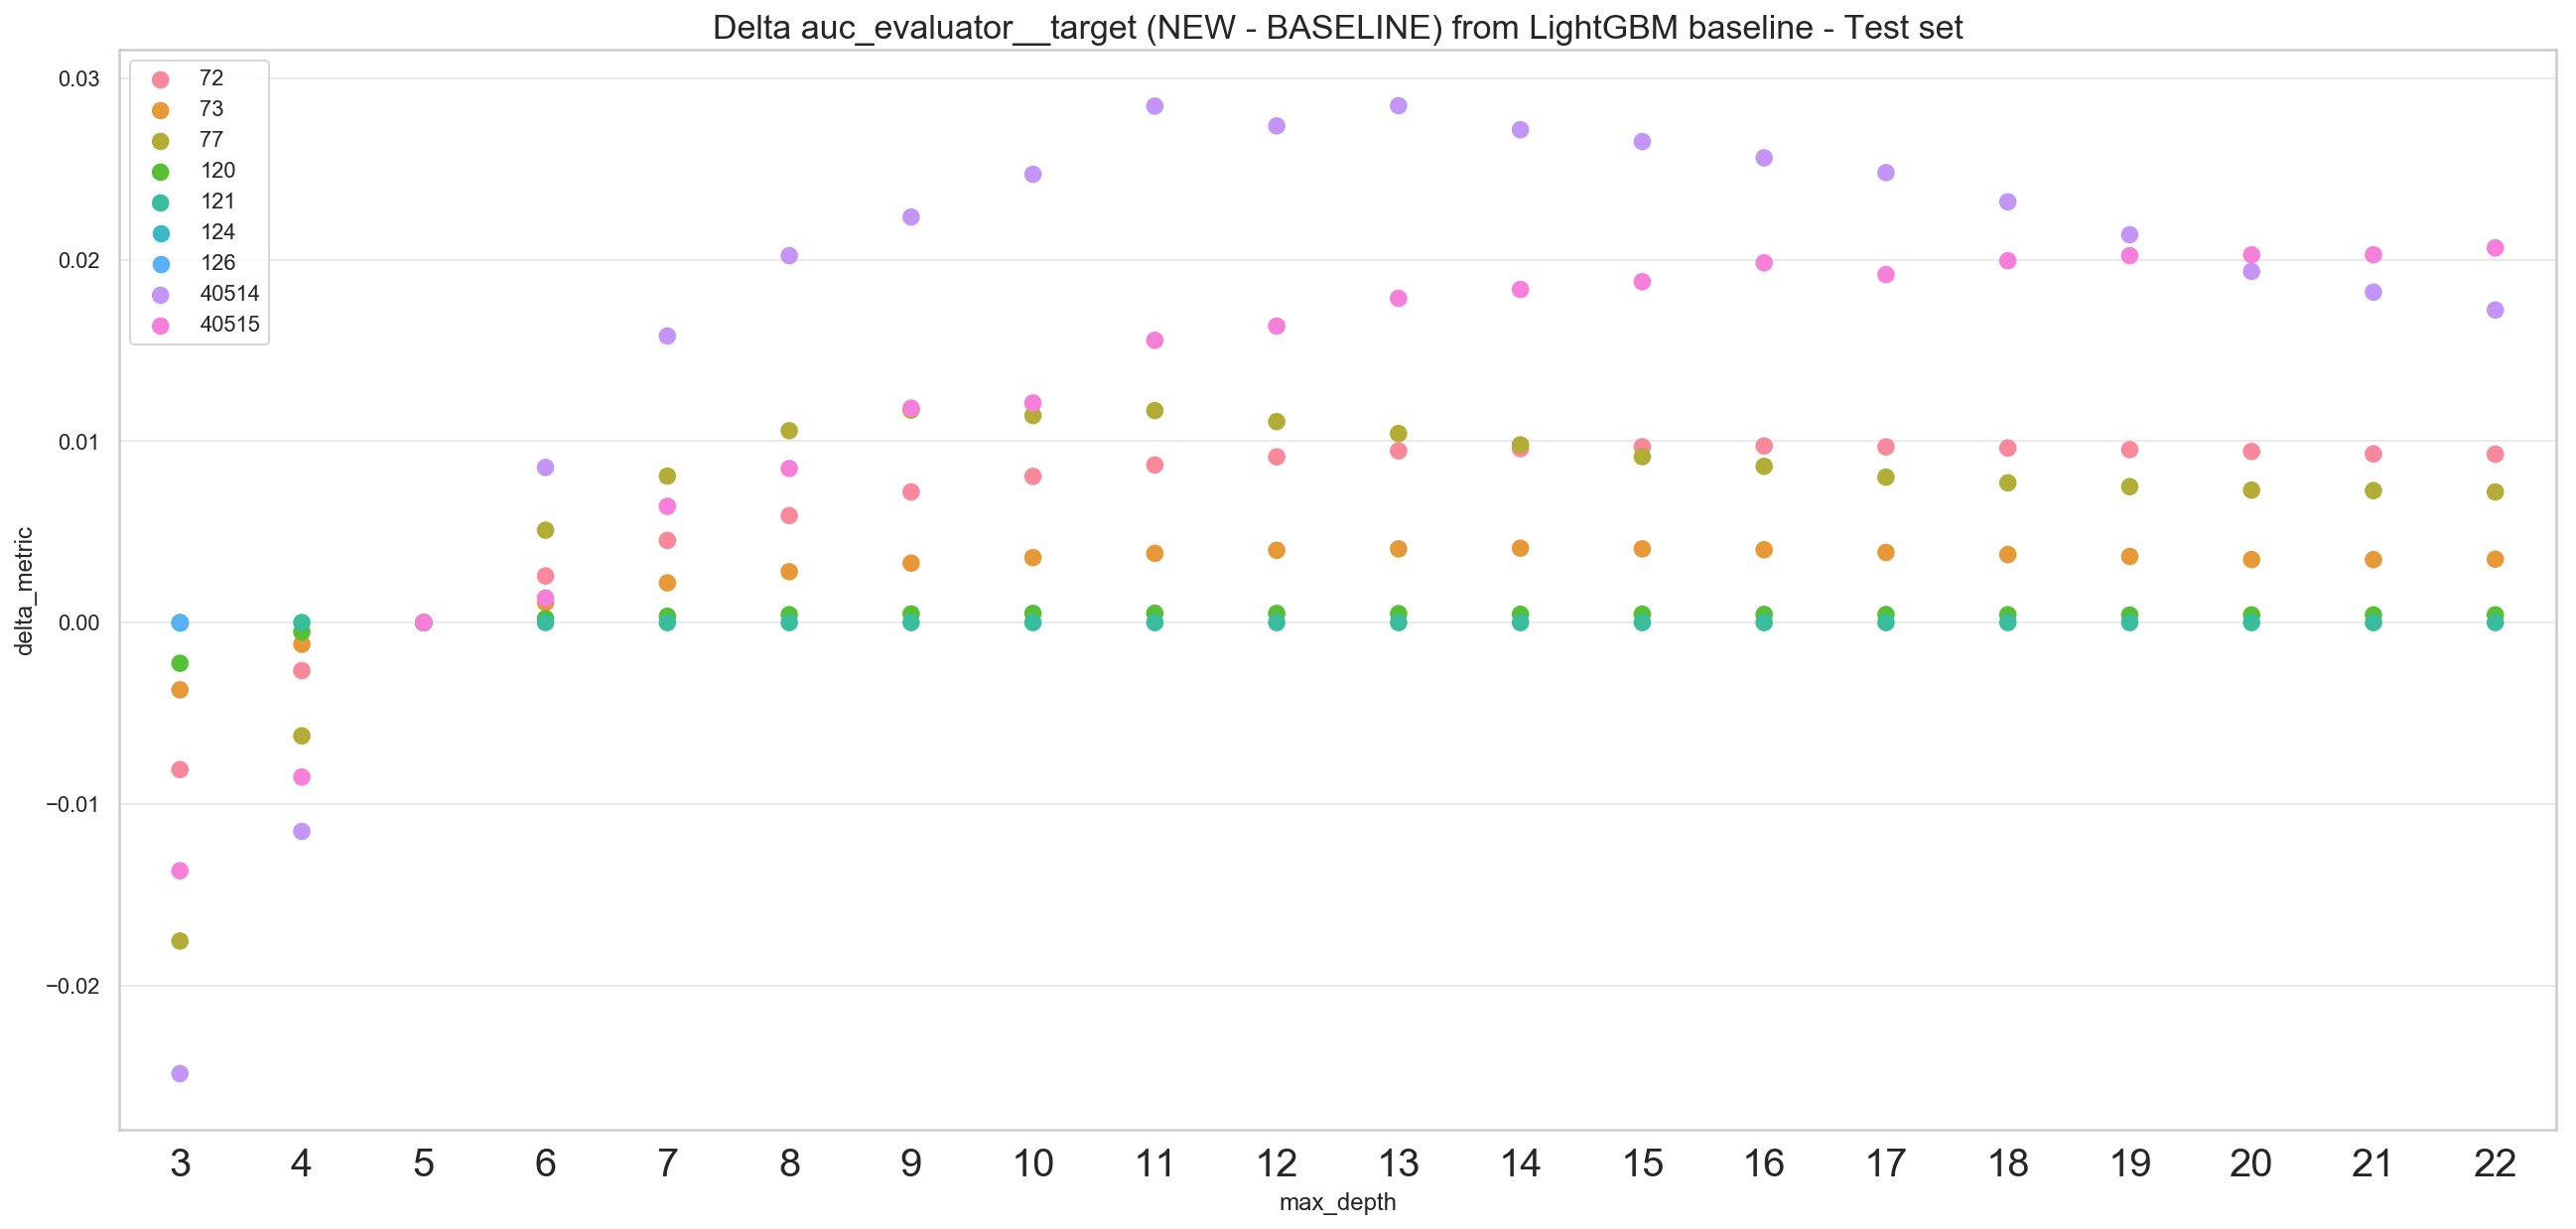
\includegraphics[width=1\textwidth]{delta_auc1.png}
    \caption{$\delta_{AUC}$ for Cluster 3, changing only \code{max\_depth}}
    \label{fig:delta-auc1}
\end{figure}


// separar em 2 capitulos:

1 - analise de metafeatures
2 - analise de sensibilidade


% \\\CONCERNS about this, and how multiple points for a given $h$, using a robust statistical test can give us more guarantee about the actual result; The study will capture mostly changes in the AUC, not if the models are already good
% thsi measure will capture the dataset sensitivity as well


% \ref{plot of a single delta metric - AUC}
% \ref{plot of a single delta metric - Brier Score}